\documentclass[12pt,a4paper,parskip=full,abstracton]{scrartcl}
\KOMAoption{bibliography}{totoc}
\KOMAoption{listof}{totoc}

\usepackage{cite}
\usepackage[pdftex]{graphicx}
\graphicspath{{graphics/}}

\usepackage[cmex10]{amsmath}
\usepackage{amssymb}
\usepackage{gensymb}
\usepackage{listings}
\usepackage{tocloft}
\usepackage{subcaption}

\usepackage{url}

\usepackage{makeidx}
\usepackage[colorlinks,hyperindex,plainpages=false,
pdftitle={High-frequency characterization of a Software Defined Radio (SDR) platform},
pdfauthor={Gernot Vormayr},
pdfsubject={Bachelor thesis},
pdfkeywords={Hochfrequenz,Software Defined Radio,SDR,GNU Radio,USRP},
pdfpagelabels,
]{hyperref}

\usepackage[binary-units,retain-explicit-plus]{siunitx}
\usepackage{pgfplots}

\pgfplotsset{compat=1.11}
\pgfplotsset{every axis plot/.append style={smooth},every axis/.append style={grid=major,legend style={font=\footnotesize}}} 

\usepgfplotslibrary{units}
\usepgfplotslibrary{fillbetween}
\pgfplotsset{unit code/.code 2 args={\si{#1#2}}}

\usepackage{tikz}
\usetikzlibrary{dsp,chains,fit,matrix,positioning,scopes,calc,backgrounds,arrows,decorations.pathmorphing,shapes.misc}
\usepackage{circuitikz}

\makeatletter

\ctikzset{rf/width/.initial=0.75}
\ctikzset{rf/height/.initial=0.75}
\ctikzset{rf/filter/sinewidth/.initial=0.8}
\ctikzset{rf/filter/sineheight/.initial=0.2}
\ctikzset{rf/switch/length/.initial=0.6}
\ctikzset{rf/adc/width/.initial=1}


\long\def\pgfrfdeclarenode#1#2#3{
    \pgfdeclareshape{#1}
    {
        \anchor{center}{
            \pgfpointorigin
        }
        \savedanchor\northwest{%
            \pgf@y=\pgfkeysvalueof{/tikz/circuitikz/bipoles/length}
            \pgf@y=\pgfkeysvalueof{/tikz/circuitikz/rf/height}\pgf@y
            \pgf@y=.5\pgf@y
            \pgf@x=\pgfkeysvalueof{/tikz/circuitikz/bipoles/length}
            \pgf@x=.5\pgf@x
            \pgf@x=-\pgfkeysvalueof{/tikz/circuitikz/rf/width}\pgf@x
        }
        \anchor{north}{
            \northwest
            \pgf@x=0pt
        }
        \anchor{south}{
            \northwest
            \pgf@x=0pt
            \pgf@y=-\pgf@y
        }
        \anchor{west}{
            \northwest
            \pgf@y=0pt
        }
        \anchor{east}{
            \northwest
            \pgf@y=0pt
            \pgf@x=-\pgf@x
        }
        \anchor{south west}{
            \northwest
            \pgf@y=-\pgf@y
        }
        \anchor{north east}{
            \northwest
            \pgf@x=-\pgf@x
        }
        \anchor{north west}{
            \northwest
        }
        \anchor{south east}{
            \northwest
            \pgf@x=-\pgf@x
            \pgf@y=-\pgf@y
        }	  
        \anchor{base}{
            \northwest
            \pgf@x=0pt	  	
        }
        \anchorborder{
            \@tempdima=\pgf@x
            \@tempdimb=\pgf@y
            \northwest
            \pgf@xa=-\pgf@x
            \pgf@ya=\pgf@y
            \pgfpointborderrectangle{\pgfpoint{\@tempdima}{\@tempdimb}}{\pgfpoint{\pgf@xa}{\pgf@ya}}
        }
        #3
        \backgroundpath{			
            \pgfsetcolor{\pgfkeysvalueof{/tikz/circuitikz/color}}	

            \northwest
            \pgf@circ@res@up = \pgf@y 
            \pgf@circ@res@down = -\pgf@y
            \pgf@circ@res@right = -\pgf@x
            \pgf@circ@res@left = \pgf@x

            \pgfscope
                \pgfsetcornersarced{\pgfpoint{4pt}{4pt}}
                \pgfpathrectanglecorners{\pgfpoint{\pgf@circ@res@left}{\pgf@circ@res@down}}{\pgfpoint{\pgf@circ@res@right}{\pgf@circ@res@up}}
                \pgfstroke
            \endpgfscope

            #2

        }
    }
}

\long\def\pgfrfdeclaremonopole#1#2{
    \pgfrfdeclarenode{#1}{#2}{
        \anchor{A}{
            \northwest
            \pgf@y=0pt
        }
    }
}

\long\def\pgfrfdeclarebipole#1#2{
    \pgfrfdeclarenode{#1}{#2}{
        \anchor{A}{
            \northwest
            \pgf@y=0pt
        }
        \anchor{B}{
            \northwest
            \pgf@y=0pt
            \pgf@x=-\pgf@x
        }
    }
}

\long\def\pgfrfdeclaretripole#1#2{
    \pgfrfdeclarenode{#1}{#2}{
        \anchor{A1}{
            \northwest
            \pgf@y=0pt
        }
        \anchor{B1}{
            \northwest
            \pgf@y=0.5\pgf@y
            \pgf@x=-\pgf@x
        }
        \anchor{B2}{
            \northwest
            \pgf@y=-0.5\pgf@y
            \pgf@x=-\pgf@x
        }
    }
}

\long\def\pgfrfdeclarequadpole#1#2{
    \pgfrfdeclarenode{#1}{#2}{
        \anchor{A1}{
            \northwest
            \pgf@y=0.5\pgf@y
        }
        \anchor{A2}{
            \northwest
            \pgf@y=-0.5\pgf@y
        }
        \anchor{B1}{
            \northwest
            \pgf@y=0.5\pgf@y
            \pgf@x=-\pgf@x
        }
        \anchor{B2}{
            \northwest
            \pgf@y=-0.5\pgf@y
            \pgf@x=-\pgf@x
        }
    }
}

\long\def\pgfrfdeclaredadc#1#2{
    \pgfdeclareshape{#1}
    {
        \anchor{center}{
            \pgfpointorigin
        }
        \savedanchor\northwest{%
            \pgf@y=\pgfkeysvalueof{/tikz/circuitikz/bipoles/length}
            \pgf@y=\pgfkeysvalueof{/tikz/circuitikz/rf/height}\pgf@y
            \pgf@y=.5\pgf@y
            \pgf@x=\pgfkeysvalueof{/tikz/circuitikz/bipoles/length}
            \pgf@x=.5\pgf@x
            \pgf@x=-\pgfkeysvalueof{/tikz/circuitikz/rf/adc/width}\pgf@x
        }
        \anchor{north}{
            \northwest
            \pgf@x=0pt
        }
        \anchor{south}{
            \northwest
            \pgf@x=0pt
            \pgf@y=-\pgf@y
        }
        \anchor{west}{
            \northwest
            \pgf@y=0pt
        }
        \anchor{east}{
            \northwest
            \pgf@y=0pt
            \pgf@x=-\pgf@x
        }
        \anchor{south west}{
            \northwest
            \pgf@y=-\pgf@y
        }
        \anchor{north east}{
            \northwest
            \pgf@x=-\pgf@x
        }
        \anchor{north west}{
            \northwest
        }
        \anchor{south east}{
            \northwest
            \pgf@x=-\pgf@x
            \pgf@y=-\pgf@y
        }	  
        \anchor{base}{
            \northwest
            \pgf@x=0pt	  	
        }
        \anchor{A}{
            \northwest
            \pgf@y=0pt
        }
        \anchor{B}{
            \northwest
            \pgf@y=0pt
            \pgf@x=-\pgf@x
        }
        \anchorborder{
            \@tempdima=\pgf@x
            \@tempdimb=\pgf@y
            \northwest
            \pgf@xa=-\pgf@x
            \pgf@ya=\pgf@y
            \pgfpointborderrectangle{\pgfpoint{\@tempdima}{\@tempdimb}}{\pgfpoint{\pgf@xa}{\pgf@ya}}
        }
        \backgroundpath{			
            \pgfsetcolor{\pgfkeysvalueof{/tikz/circuitikz/color}}	

            \northwest
            \pgf@circ@res@up = \pgf@y 
            \pgf@circ@res@down = -\pgf@y
            \pgf@circ@res@right = -\pgf@x
            \pgf@circ@res@left = \pgf@x

            #2

        }
    }
}

\pgfrfdeclarebipole{attenuator}{
    \pgfscope             
        \pgftransformscale{.5}
        \pgfnode{resistorshape}{center}{}{pgf@att}{\pgfusepath{stroke}}
    \endpgfscope
    \pgfpathmoveto{\pgfpoint{\pgf@circ@res@left}{0}}
    \pgfpathlineto{\pgfpointanchor{pgf@att}{b}}
    \pgfpathmoveto{\pgfpoint{\pgf@circ@res@right}{0}}
    \pgfpathlineto{\pgfpointanchor{pgf@att}{a}}
    \pgfusepath{draw}

}

\pgfrfdeclarebipole{vattenuator}{
    \pgfscope             
        \pgftransformscale{.5}
        \pgfnode{resistorshape}{center}{}{pgf@att}{\pgfusepath{stroke}}
    \endpgfscope
    \pgfpathmoveto{\pgfpoint{\pgf@circ@res@left}{0}}
    \pgfpathlineto{\pgfpointanchor{pgf@att}{b}}
    \pgfpathmoveto{\pgfpoint{\pgf@circ@res@right}{0}}
    \pgfpathlineto{\pgfpointanchor{pgf@att}{a}}
    \pgfusepath{draw}
    \pgfpathmoveto{\pgfpoint{0.5\pgf@circ@res@left}{0.7\pgf@circ@res@down}}
    \pgfpathlineto{\pgfpoint{0.5\pgf@circ@res@right}{0.7\pgf@circ@res@up}}
    \pgfsetarrowsend{stealth}
    \pgfusepath{draw}
}

\def\pgfrffiltersinewave{
        \pgfpathmoveto{\pgfpoint{\pgf@xb}{\pgf@yb}}
        \pgfpathsine{\pgfpoint{\pgf@xa}{\pgf@ya}}
        \pgfpathcosine{\pgfpoint{\pgf@xa}{-\pgf@ya}}
        \pgfpathsine{\pgfpoint{\pgf@xa}{-\pgf@ya}}
        \pgfpathcosine{\pgfpoint{\pgf@xa}{\pgf@ya}}
        \advance \pgf@yb by \pgf@circ@res@step
}

\long\def\pgfrfdeclarefilter#1#2{
    \pgfrfdeclarebipole{#1}{
        \pgfscope
            \pgf@yb = 0.5\pgf@circ@res@up
            \pgf@circ@res@step = -0.5\pgf@circ@res@up
            
            \pgf@xa = \ctikzvalof{rf/filter/sinewidth}\pgf@circ@res@right
            \divide \pgf@xa by 2
            \pgf@ya = \ctikzvalof{rf/filter/sineheight}\pgf@circ@res@up
            \pgf@xb = \ctikzvalof{rf/filter/sinewidth}\pgf@circ@res@left

            \pgfrffiltersinewave
            \pgfrffiltersinewave
            \pgfrffiltersinewave
            \pgfstroke
        \endpgfscope
        #2
    }
}

\def\pgfrfstrikewave#1{
    \pgf@ya = 0.5\pgf@circ@res@up
    \pgf@yb = #1\pgf@ya
    \advance \pgf@ya by -\pgf@yb
    \advance \pgf@ya by -2pt
    \pgfpathmoveto{\pgfpoint{-2pt}{\pgf@ya}}
    \advance \pgf@ya by 4pt
    \pgfpathlineto{\pgfpoint{2pt}{\pgf@ya}}
}

\pgfrfdeclarefilter{lowpass}{
    \pgfrfstrikewave{0}
    \pgfrfstrikewave{1}
    \pgfusepath{draw}
}

\pgfrfdeclarefilter{highpass}{
    \pgfrfstrikewave{1}
    \pgfrfstrikewave{2}
    \pgfusepath{draw}
}

\pgfrfdeclarefilter{bandpass}{
    \pgfrfstrikewave{0}
    \pgfrfstrikewave{2}
    \pgfusepath{draw}
}

\pgfrfdeclaretripole{altswitch}{
    \pgf@xa = \ctikzvalof{rf/switch/length}\pgf@circ@res@left
    \pgfpathmoveto{\pgfpoint{\pgf@circ@res@left}{0}}
    \pgfpathlineto{\pgfpoint{\pgf@xa}{0}}
    \pgfpathlineto{\pgfpoint{-\pgf@xa}{-0.5\pgf@circ@res@up}}
    \pgfpathlineto{\pgfpoint{\pgf@circ@res@right}{-0.5\pgf@circ@res@up}}
    \pgfpathmoveto{\pgfpoint{\pgf@circ@res@right}{0.5\pgf@circ@res@up}}
    \pgfpathlineto{\pgfpoint{-\pgf@xa}{0.5\pgf@circ@res@up}}
    \pgfusepath{draw}
    \pgfpathcircle{\pgfpoint{-\ctikzvalof{rf/switch/length}\pgf@circ@res@left}{-0.5\pgf@circ@res@up}}{1.5pt}
    \pgfusepath{draw,fill}
    \pgfsetfillcolor{white}
    \pgfpathcircle{\pgfpoint{-\ctikzvalof{rf/switch/length}\pgf@circ@res@left}{0.5\pgf@circ@res@up}}{1.5pt}
    \pgfusepath{draw,fill}
    \pgfpathmoveto{\pgfpoint{0}{0.25\pgf@circ@res@down}}
    \pgfmathsetmacro{\tikz@start@angle@temp}{(atan2(0.5*\the\pgf@circ@res@up,2*\ctikzvalof{rf/switch/length}*\the\pgf@circ@res@right))}
    \pgfpatharc{-\tikz@start@angle@temp}{+\tikz@start@angle@temp}{\ctikzvalof{rf/switch/length}\pgf@circ@res@right}
    \pgfsetarrowsend{stealth}
    \pgfusepath{draw}
}

\pgfrfdeclarequadpole{chswitch}{
    \pgf@xa = \ctikzvalof{rf/switch/length}\pgf@circ@res@left
    \pgfpathmoveto{\pgfpoint{\pgf@circ@res@left}{0.5\pgf@circ@res@up}}
    \pgfpathlineto{\pgfpoint{\pgf@circ@res@right}{0.5\pgf@circ@res@up}}
    \pgfpathmoveto{\pgfpoint{\pgf@circ@res@left}{0.5\pgf@circ@res@down}}
    \pgfpathlineto{\pgfpoint{\pgf@circ@res@right}{0.5\pgf@circ@res@down}}
    \pgfusepath{draw}
    \pgfpathmoveto{\pgfpoint{\ctikzvalof{rf/switch/length}\pgf@circ@res@left}{0.5\pgf@circ@res@up}}{1.5pt}
    \pgfpathlineto{\pgfpoint{\ctikzvalof{rf/switch/length}\pgf@circ@res@right}{0.5\pgf@circ@res@down}}{1.5pt}
    \pgfpathmoveto{\pgfpoint{\ctikzvalof{rf/switch/length}\pgf@circ@res@right}{0.5\pgf@circ@res@up}}{1.5pt}
    \pgfpathlineto{\pgfpoint{\ctikzvalof{rf/switch/length}\pgf@circ@res@left}{0.5\pgf@circ@res@down}}{1.5pt}
    \pgfsetdash{{3pt}{2pt}}{0pt}
    \pgfusepath{draw}
    \pgfsetfillcolor{white}
    \pgfsetdash{}{0pt}
    \pgfpathcircle{\pgfpoint{\ctikzvalof{rf/switch/length}\pgf@circ@res@left}{0.5\pgf@circ@res@up}}{1.5pt}
    \pgfpathcircle{\pgfpoint{\ctikzvalof{rf/switch/length}\pgf@circ@res@left}{0.5\pgf@circ@res@down}}{1.5pt}
    \pgfpathcircle{\pgfpoint{\ctikzvalof{rf/switch/length}\pgf@circ@res@right}{0.5\pgf@circ@res@up}}{1.5pt}
    \pgfpathcircle{\pgfpoint{\ctikzvalof{rf/switch/length}\pgf@circ@res@right}{0.5\pgf@circ@res@down}}{1.5pt}
    \pgfusepath{draw,fill}
}

\pgfrfdeclaredadc{adc}{
    \pgf@xa=\pgf@circ@res@left
    \divide \pgf@xa by 3
    \pgfpathmoveto{\pgfpoint{\pgf@circ@res@left}{0pt}}
    \pgfpathlineto{\pgfpoint{\pgf@xa}{\pgf@circ@res@up}}
    \pgfpathlineto{\pgfpoint{\pgf@circ@res@right}{\pgf@circ@res@up}}
    \pgfpathlineto{\pgfpoint{\pgf@circ@res@right}{\pgf@circ@res@down}}
    \pgfpathlineto{\pgfpoint{\pgf@xa}{\pgf@circ@res@down}}
    \pgfclosepath
    \pgfusepath{draw}
}

\pgfrfdeclaredadc{dac}{
    \pgf@xa=\pgf@circ@res@right
    \divide \pgf@xa by 3
    \pgfpathmoveto{\pgfpoint{\pgf@circ@res@right}{0pt}}
    \pgfpathlineto{\pgfpoint{\pgf@xa}{\pgf@circ@res@up}}
    \pgfpathlineto{\pgfpoint{\pgf@circ@res@left}{\pgf@circ@res@up}}
    \pgfpathlineto{\pgfpoint{\pgf@circ@res@left}{\pgf@circ@res@down}}
    \pgfpathlineto{\pgfpoint{\pgf@xa}{\pgf@circ@res@down}}
    \pgfclosepath
    \pgfusepath{draw}
}

\pgfrfdeclarebipole{amp}{
    \pgfscope             
        \pgftransformscale{.5}
        \pgfnode{buffer}{center}{}{pgf@amp}{\pgfusepath{stroke}}
    \endpgfscope
    \pgfpathmoveto{\pgfpoint{\pgf@circ@res@left}{0}}
    \pgfpathlineto{\pgfpointanchor{pgf@amp}{in}}
    \pgfpathmoveto{\pgfpoint{\pgf@circ@res@right}{0}}
    \pgfpathlineto{\pgfpointanchor{pgf@amp}{out}}
    \pgfusepath{draw}
}

\pgfrfdeclarenode{iqmix}{
    \pgfscope             
        \pgftransformshift{\pgfpoint{0.5\pgf@circ@res@right}{0.5\pgf@circ@res@up}}
        \pgftransformrotate{180}
        \pgftransformscale{.2}
        \pgfnode{mixer}{center}{}{pgf@mixi}{\pgfusepath{stroke}}
    \endpgfscope
    \pgfscope             
        \pgftransformshift{\pgfpoint{0}{0.5\pgf@circ@res@down}}
        \pgftransformrotate{180}
        \pgftransformscale{.2}
        \pgfnode{mixer}{center}{}{pgf@mixq}{\pgfusepath{stroke}}
    \endpgfscope
    \pgfscope             
        \pgftransformscale{.35}
        \pgfnode{rectangle}{center}{$90\degree$}{pgf@phase}{\pgfusepath{stroke}}
    \endpgfscope
    \pgfpathmoveto{\pgfpoint{\pgf@circ@res@left}{0pt}}
    \pgfpathlineto{\pgfpoint{0.6\pgf@circ@res@left}{0pt}}
    \pgfpathlineto{\pgfpoint{0.6\pgf@circ@res@left}{0.5\pgf@circ@res@up}}
    \pgfpathlineto{\pgfpointanchor{pgf@mixi}{out}}
    \pgfpathmoveto{\pgfpoint{0.6\pgf@circ@res@left}{0pt}}
    \pgfpathlineto{\pgfpoint{0.6\pgf@circ@res@left}{0.5\pgf@circ@res@down}}
    \pgfpathlineto{\pgfpointanchor{pgf@mixq}{out}}
    \pgfpathmoveto{\pgfpointanchor{pgf@mixi}{in}}
    \pgfpathlineto{\pgfpoint{\pgf@circ@res@right}{0.5\pgf@circ@res@up}}
    \pgfpathmoveto{\pgfpointanchor{pgf@mixq}{in}}
    \pgfpathlineto{\pgfpoint{\pgf@circ@res@right}{0.5\pgf@circ@res@down}}
    \pgfpathmoveto{\pgfpoint{0pt}{\pgf@circ@res@up}}
    \pgfpathlineto{\pgfpointanchor{pgf@phase}{north}}
    \pgfpathmoveto{\pgfpointanchor{pgf@phase}{south}}
    \pgfpathlineto{\pgfpointanchor{pgf@mixq}{in 2}}
    \pgfpathmoveto{\pgfpoint{0pt}{0.8\pgf@circ@res@up}}
    \pgfpathlineto{\pgfpoint{0.5\pgf@circ@res@right}{0.8\pgf@circ@res@up}}
    \pgfpathlineto{\pgfpointanchor{pgf@mixi}{in 2}}
    \pgfusepath{draw}
    \pgfpathcircle{\pgfpoint{0pt}{0.8\pgf@circ@res@up}}{1pt}
    \pgfpathcircle{\pgfpoint{0.6\pgf@circ@res@left}{0pt}}{1pt}
    \pgfusepath{fill}

}{
    \anchor{A1}{
        \northwest
        \pgf@y=0pt
    }
    \anchor{B1}{
        \northwest
        \pgf@y=0.5\pgf@y
        \pgf@x=-\pgf@x
    }
    \anchor{B2}{
        \northwest
        \pgf@y=-0.5\pgf@y
        \pgf@x=-\pgf@x
    }
    \anchor{C1}{
        \northwest
        \pgf@x=0pt
    }
}

\pgfrfdeclarenode{iqmixdown}{
    \pgfscope             
        \pgftransformshift{\pgfpoint{0.5\pgf@circ@res@right}{0.5\pgf@circ@res@down}}
        \pgftransformscale{.2}
        \pgfnode{mixer}{center}{}{pgf@mixi}{\pgfusepath{stroke}}
    \endpgfscope
    \pgfscope             
        \pgftransformshift{\pgfpoint{0}{0.5\pgf@circ@res@up}}
        \pgftransformscale{.2}
        \pgfnode{mixer}{center}{}{pgf@mixq}{\pgfusepath{stroke}}
    \endpgfscope
    \pgfscope             
        \pgftransformscale{.35}
        \pgfnode{rectangle}{center}{$90\degree$}{pgf@phase}{\pgfusepath{stroke}}
    \endpgfscope
    \pgfpathmoveto{\pgfpoint{\pgf@circ@res@left}{0pt}}
    \pgfpathlineto{\pgfpoint{0.6\pgf@circ@res@left}{0pt}}
    \pgfpathlineto{\pgfpoint{0.6\pgf@circ@res@left}{0.5\pgf@circ@res@down}}
    \pgfpathlineto{\pgfpointanchor{pgf@mixi}{in}}
    \pgfpathmoveto{\pgfpoint{0.6\pgf@circ@res@left}{0pt}}
    \pgfpathlineto{\pgfpoint{0.6\pgf@circ@res@left}{0.5\pgf@circ@res@up}}
    \pgfpathlineto{\pgfpointanchor{pgf@mixq}{in}}
    \pgfpathmoveto{\pgfpointanchor{pgf@mixi}{out}}
    \pgfpathlineto{\pgfpoint{\pgf@circ@res@right}{0.5\pgf@circ@res@down}}
    \pgfpathmoveto{\pgfpointanchor{pgf@mixq}{out}}
    \pgfpathlineto{\pgfpoint{\pgf@circ@res@right}{0.5\pgf@circ@res@up}}
    \pgfpathmoveto{\pgfpoint{0pt}{\pgf@circ@res@down}}
    \pgfpathlineto{\pgfpointanchor{pgf@phase}{south}}
    \pgfpathmoveto{\pgfpointanchor{pgf@phase}{north}}
    \pgfpathlineto{\pgfpointanchor{pgf@mixq}{in 2}}
    \pgfpathmoveto{\pgfpoint{0pt}{0.8\pgf@circ@res@down}}
    \pgfpathlineto{\pgfpoint{0.5\pgf@circ@res@right}{0.8\pgf@circ@res@down}}
    \pgfpathlineto{\pgfpointanchor{pgf@mixi}{in 2}}
    \pgfusepath{draw}
    \pgfpathcircle{\pgfpoint{0pt}{0.8\pgf@circ@res@down}}{1pt}
    \pgfpathcircle{\pgfpoint{0.6\pgf@circ@res@left}{0pt}}{1pt}
    \pgfusepath{fill}

}{
    \anchor{A1}{
        \northwest
        \pgf@y=0pt
    }
    \anchor{B1}{
        \northwest
        \pgf@y=0.5\pgf@y
        \pgf@x=-\pgf@x
    }
    \anchor{B2}{
        \northwest
        \pgf@y=-0.5\pgf@y
        \pgf@x=-\pgf@x
    }
    \anchor{C1}{
        \northwest
        \pgf@x=0pt
        \pgf@y=-\pgf@y
    }
}

\pgfrfdeclarebipole{pll}{
    \pgftext{PLL}
}
\pgfrfdeclarebipole{dut}{
    \pgftext{DUT}
}

\pgfrfdeclaremonopole{generator}{
    \pgfscope             
        \pgftransformscale{.5}
        \pgftransformrotate{90}
        \pgfnode{vsourcesinshape}{center}{}{pgf@att}{\pgfusepath{stroke}}
    \endpgfscope
}

\pgfrfdeclaremonopole{powermeter}{
    \pgfscope             
        \pgftransformscale{.5}
        \pgftransformrotate{-90}
        \pgfnode{fulldiodeshape}{center}{}{pgf@att}{\pgfusepath{stroke}}
    \endpgfscope
    \pgfpathmoveto{\pgfpoint{0pt}{0.7\pgf@circ@res@up}}
    \pgfpathlineto{\pgfpoint{0pt}{0.7\pgf@circ@res@down}}
    \pgfusepath{draw}
}

\makeatother


\makeatletter
\pgfdeclareshape{dspswitchshape}{%
    \inheritsavedanchors[from=rectangle]
    \inheritanchorborder[from=rectangle]
    \inheritanchor[from=rectangle]{north}
    \inheritanchor[from=rectangle]{north west}
    \inheritanchor[from=rectangle]{north east}
    \inheritanchor[from=rectangle]{center}
    \inheritanchor[from=rectangle]{west}
    \inheritanchor[from=rectangle]{east}
    \inheritanchor[from=rectangle]{mid}
    \inheritanchor[from=rectangle]{mid west}
    \inheritanchor[from=rectangle]{mid east}
    \inheritanchor[from=rectangle]{base}
    \inheritanchor[from=rectangle]{base west}
    \inheritanchor[from=rectangle]{base east}
    \inheritanchor[from=rectangle]{south}
    \inheritanchor[from=rectangle]{south west}
    \inheritanchor[from=rectangle]{south east}
    \backgroundpath{%
      \pgfpathrectanglecorners
      {\pgfpointadd{\southwest}{\pgfpoint{\pgfkeysvalueof{/pgf/outer xsep}}{\pgfkeysvalueof{/pgf/outer ysep}}}}
      {\pgfpointadd{\northeast}{\pgfpointscale{-1}{\pgfpoint{\pgfkeysvalueof{/pgf/outer xsep}}{\pgfkeysvalueof{/pgf/outer ysep}}}}}
      \southwest \pgf@xa=\pgf@x \pgf@ya=\pgf@y
      \northeast \pgf@xb=\pgf@x \pgf@yb=\pgf@y
      \advance\pgf@xa by 6pt
      \advance\pgf@xb by -6pt
      \advance\pgf@yb by -7pt
      \advance\pgf@ya by 7pt
      {%
          \pgfpathmoveto{\pgfpoint{\pgf@xa}{\pgf@yb}}
          \pgfpathlineto{\pgfpoint{\pgf@xb}{\pgf@yb}}
          \pgfpathmoveto{\pgfpoint{\pgf@xa}{\pgf@ya}}
          \pgfpathlineto{\pgfpoint{\pgf@xb}{\pgf@ya}}
          \pgfusepath{stroke}
          \pgfpathmoveto{\pgfpoint{\pgf@xb}{\pgf@yb}}
          \pgfpathlineto{\pgfpoint{\pgf@xa}{\pgf@ya}}
          \pgfpathmoveto{\pgfpoint{\pgf@xb}{\pgf@ya}}
          \pgfpathlineto{\pgfpoint{\pgf@xa}{\pgf@yb}}
          \pgfsetdash{{0.5pt}{2pt}}{0pt}
          \pgfusepath{stroke}
      }
      {\pgfpathcircle{\pgfpoint{\pgf@xa}{\pgf@yb}}{2pt}}
      {\pgfpathcircle{\pgfpoint{\pgf@xb}{\pgf@yb}}{2pt}}
      {\pgfpathcircle{\pgfpoint{\pgf@xa}{\pgf@ya}}{2pt}}
      {\pgfpathcircle{\pgfpoint{\pgf@xb}{\pgf@ya}}{2pt}}
      \pgfsetdash{}{0pt}
      \color{white}
      \pgfsetstrokecolor{black} 
      \pgfusepath{fill,stroke}
    }
}
\makeatother
\tikzset{dspswitch/.style={shape=dspswitchshape,draw,align=center,text depth=0.3em,text height=1em,inner sep=0pt,
         line cap=round,line join=round,line width=\dsplinewidth,minimum size=\dspsquareblocksize}}

\tikzset{bitwidth/.style n args={2}{strike out,draw,label={[label distance=-1mm]#1:\tiny#2},scale=0.5}}

\usepgfplotslibrary{external}
\tikzexternalize[mode=list and make]
\tikzsetexternalprefix{figures/}

\DeclareSIUnit \belm {Bm}
\DeclareSIUnit \belfs {BFS}
\DeclareSIUnit \samples {S}
\sisetup{per-mode = symbol}

\lstset{language=Python,numbers=left,numberstyle=\tiny,stepnumber=5,numbersep=5pt,frame=single,
breaklines=true,postbreak=\raisebox{0ex}[0ex][0ex]{\ensuremath{\color{red}\hookrightarrow\space}},
captionpos=b,escapeinside={(*}{*)}}

\usepackage[noabbrev]{cleveref}

\usepackage{placeins}

\usepackage[acronym]{glossaries}

\newacronym{usrp}{USRP}{Universal Software Radio Platform}
\newacronym{sdr}{SDR}{software defined radio}
\newacronym{adc}{ADC}{analog-to-digital converter}
\newacronym{dac}{DAC}{digital-to-analog converter}
\newacronym{dsp}{DSP}{digital signal processor}
\newacronym{fpga}{FPGA}{field programmable gate array}
\newacronym{ni}{NI}{National Instruments}
\newacronym{rx}{RX}{receive}
\newacronym{tx}{TX}{transmit}
\newacronym{lo}{LO}{local oscillator}
\newacronym{pll}{PLL}{phase-locked loop}
\newacronym{lna}{LNA}{low noise amplifier}
\newacronym{dc}{DC}{direct current}
\newacronym{ac}{AC}{alternating current}
\newacronym{iq}{IQ}{in-phase/quadrature-phase}
\newacronym{ddc}{DDC}{digital down-converter}
\newacronym{duc}{DUC}{digital up-converter}
\newacronym[longplural={electrically erasable programmable read-only memories}]{eeprom}{EEPROM}{electrically erasable programmable read-only memory}
\newacronym[longplural={general-purpose inputs/outputs}]{gpio}{GPIO}{general-purpose input/output}
\newacronym{cordic}{CORDIC}{coordinate rotation digital computer}
\newacronym{cic}{CIC}{cascaded integrator-comb}
\newacronym{fir}{FIR}{finite impulse response}
\newacronym{fifo}{FIFO}{first in first out}
\newacronym{uhd}{uhd}{\Glsentryshort{usrp} hardware driver}
\newacronym{volk}{VOLK}{vector-optimized library of kernels}
\newacronym{gui}{GUI}{graphical user interface}
\newacronym{ui}{UI}{user interface}
\newacronym{rf}{RF}{radio frequency}
\newacronym{if}{IF}{intermediate frequency}
\newacronym{ram}{RAM}{random access memory}
\makeglossaries

\newcommand*\rot{\rotatebox{90}}
\newcommand*\X{$\times$}

\usepackage{booktabs}

\begin{document}
\begin{titlepage}
    \enlargethispage{1cm}
    \centering
    %\begin{minipage}{0.49\linewidth}
    %    
\includegraphics[height=1.5cm,keepaspectratio]{EMCE_Logo_CMYK_color}
    %\end{minipage}
    %\begin{minipage}{0.49\linewidth}
    %    \flushright
    %    
\includegraphics[height=1.5cm,keepaspectratio]{TULogo_CMYK}
    %\end{minipage}\\
    \vspace*{5cm}
    {\Huge \textbf{Bachelor thesis}}\\
    \vspace*{1cm}
    {\Large High-frequency characterization of a \gls{sdr} platform}

    \vspace*{2cm}
    {\large Gernot ~\textsc{Vormayr} ~\\ 0425210 } ~\\ 

    \vspace*{2cm}
    {\today } ~\\ 

    \vfill
    {Supervisors} ~\\\vspace*{0.1cm}
    {Ass.Prof. Dipl.-Ing. Dr.techn. \large Holger ~\textsc{Arthaber}} ~\\
    {Univ.Ass. Dipl.-Ing. Dr.techn. \large Thomas ~\textsc{Faseth}}
    \vspace*{2cm}

    \rule{\linewidth}{0.4pt}
    \begin{minipage}[t]{0.55\linewidth}
        \flushleft
        \begin{large}
            EMCE - Institute of Electrodynamics, Microwave and Circuit Engineering
        \end{large}\\
        Vienna University of Technology
    \end{minipage}
    \hfill
    \begin{minipage}[t]{0.27\linewidth}
        \flushright
        Gusshausstrasse 25\\
        1040 Vienna\\
        www.emce.tuwien.ac.at
    \end{minipage}
    \vspace*{-3pt}
    \rule{\linewidth}{0.4pt}
    \clearpage
\end{titlepage}

\tableofcontents
\clearpage
\begin{abstract}
The software defined radio platform characterized in this bachelor thesis is the Ettus
Research \gls{usrp}. The characterization consists of a \gls{rf} response,
a \gls{if} response and the intermodulation properties. The small signal
behaviour and compression effects are described with the frequency responses. Nonlinearities
are characterized by the intermodulation properties. With these results the characteristics
of the hardware can be taken into account during the design process of radio transceivers.
This is especially important for high performance radio systems, which can be affected by
nonlinearities and deviations from the specifications.

This work starts with a full description of the inner workings of the analog and
the digital part of the platform, which was elaborated from the freely available
source codes. After this GNU Radio and Matlab scripts, to automate the measurements, were
developed. GNU Radio usage is described in this work based on these scripts. The
processed results, measurement setups, and discussions can be found in
the second section of this work. The third section contains a summary, conclusions and ideas for further work.

\end{abstract}
\clearpage
\section{Introduction}
\Gls{sdr} systems can be operated on a very broad frequency range,
easily adapted to various needs, and allow operations which would be almost
impossible or very expensive in analog hardware. A \gls{sdr} consists of specialised
software, a general purpose computer, an analog frontend with fast
\glspl{adc}/\glspl{dac}, an optional \gls{dsp}, and frequency correction capabilities.

One of those frontends is 
the Ettus Research \gls{usrp} N2x0 product family. This family consists of the N200 and
the N210, of which the latter has a superior \gls{fpga}, allowing additional custom \gls{dsp} code directly
in the device. Both contain \SI{100}{\mega\samples\per\second} dual \glspl{adc},
\SI{400}{\mega\samples\per\second} dual \glspl{dac}, a Xilinx Spartan
3A-DSP \gls{fpga}, and Gigabit Ethernet connectivity to stream data. The analog part is
provided by an interchangable family of daughter boards, which allow operation from
\gls{dc} to \SI{6}{\giga\hertz}\cite{ettus_n2x0}. These products are also available as rebranded
versions from \gls{ni}.
\subsection{\Glsentryshort{ni} \Glsentryshort{usrp}-2922}
\label{sec:usrp}
\begin{figure}[htb]
\resizebox{\linewidth}{!}{
\begin{tikzpicture}[node distance=0.6]
    \tikzstyle{every node}=[font=\footnotesize]
    \draw node[dspnodeopen,label=above:RX] (rx) {};
    \draw node[amp,right=of rx,label=above:LNA1] (lna1) {};
    \draw node[altswitch,right=of lna1,anchor=B2,label=below:SW2,rotate=180] (sw2) {};
    \draw node[vattenuator,right=of sw2.west,label={[fill=white]above:ATT1}] (att1) {};
    \draw node[amp,right=of att1,label=above:LNA2] (lna2) {};
    \draw node[iqmix,right=of lna2,label=below:DEMOD] (demod) {};
    \draw node[lowpass,right=of demod.north east,label=above:LP2,yshift=1mm] (lp2a) {};
    \draw node[lowpass,right=of demod.south east,label=below:\scriptsize\SI{20}{\mega\hertz},yshift=-1mm] (lp2b) {};
    \draw node[amp,right=of lp2a,label=above:AMP1] (amp1a) {};
    \draw node[amp,right=of lp2b] (amp1b) {};
    \draw node[lowpass,right=of amp1a,label=above:LP3] (lp3a) {};
    \draw node[lowpass,right=of amp1b,label=below:\scriptsize\SI{50}{\mega\hertz}] (lp3b) {};
    \draw node[adc,right=of lp3a,label=above:ADC] (adca) {};
    \draw node[adc,right=of lp3b] (adcb) {};
    \draw node[chswitch,above=1.5 of demod,rotate=90,anchor=A2] (sw1) {};
    \draw node[rotate=90,anchor=south] at (sw1.north) {SW1};
    \draw node[lowpass,left=1 of sw1.north,rotate=90,anchor=south] (lp1) {};
    \draw node[rotate=90,anchor=south] at (lp1.north) {LP1};
    \draw node[rotate=90,anchor=north] at (lp1.south) {\scriptsize\SI{1.2}{\giga\hertz}};
    \draw node[pll,above=1.8 of lp3a,label=above:SYNTH1] (synth1) {};
    
    \draw node[dspnodeopen,label=above:TX/RX,below=3.5 of rx] (tx) {};
    \draw node[altswitch,right=of tx,label=above:SW3] (sw3) {};
    \draw ($(sw3)!.5!(sw2)$) node[amp,rotate=90] (lna3) {};
    \draw node[rotate=90,anchor=south] at (lna3.north) {LNA3};
    \draw node[lowpass,right=of sw3.B2,label=above:LP4,label=below:\scriptsize\SI{5.8}{\giga\hertz}] (lp4) {};
    \draw node[amp,right=of lp4,rotate=180,label=below:AMP2,anchor=B] (amp2) {};
    \draw node[vattenuator,right=of amp2.A,label={[fill=white]above:ATT2}] (att2) {};
    \draw node[amp,right=of att2,rotate=180,label=below:AMP3,anchor=B] (amp3) {};
    \draw node[attenuator,right=of amp3.A,label=above:ATT3] (att3) {};
    \draw node[iqmixdown,right=of att3,label=above:MOD] (mod) {};
    \draw node[lowpass,right=of mod.north east,label=above:LP5,yshift=1mm] (lp5a) {};
    \draw node[lowpass,right=of mod.south east,label=below:\scriptsize\SI{20}{\mega\hertz},yshift=-1mm] (lp5b) {};
    \draw node[dac,right=of lp5a,label=above:DAC] (daca) {};
    \draw node[dac,right=of lp5b] (dacb) {};
    \draw node[chswitch,below=1.5 of mod,rotate=90,anchor=B2] (sw4) {};
    \draw node[rotate=90,anchor=south] at (sw4.north) {SW4};
    \draw node[lowpass,left=1 of sw4.north,rotate=90,anchor=south] (lp6) {};
    \draw node[rotate=90,anchor=south] at (lp6.north) {LP6};
    \draw node[rotate=90,anchor=north] at (lp6.south) {\scriptsize\SI{1.2}{\giga\hertz}};
    \draw node[pll,below=1.8 of lp5b,label=above:SYNTH2] (synth2) {};


    \draw (rx) -- (lna1) -- (sw2.B2);
    \draw (sw2.A1) -- (att1) -- (lna2) -- (demod);
    \draw (demod.B1) -| ($(demod)!.5!(lp2a)$) |- (lp2a) -- (amp1a) -- (lp3a);
    \draw (lp3a) [decoration={markings,mark=at position 0.7 with {\arrow{triangle 45}}},postaction={decorate}] -- (adca.A);
    \draw (demod.B2) -| ($(demod)!.5!(lp2b)$) |- (lp2b) -- (amp1b) -- (lp3b);
    \draw (lp3b) [decoration={markings,mark=at position 0.7 with {\arrow{triangle 45}}},postaction={decorate}] -- (adcb.A);
    \draw (demod.C1) -- (sw1.A2);
    \draw (sw1.A1) |- ($(lp1.A) - (0,0.4)$) -- (lp1.A);
    \draw (sw1.B1) |- ($(lp1.B) + (0,0.4)$) -- (lp1.B);
    \draw (sw1.B2) |- (synth1);

    \draw (tx) -- (sw3);
    \draw (sw3.B1) -| (lna3) |- (sw2.B1);
    \draw (sw3.B2) -- (lp4) -- (amp2) -- (amp2) -- (att2) -- (amp3) -- (att3) -- (mod);
    \draw (mod.B1) -| ($(mod)!.5!(lp5a)$) |- (lp5a);
    \draw (lp5a) [decoration={markings,mark=at position 0.3 with {\arrowreversed{triangle 45}}},postaction={decorate}] -- (daca.A);
    \draw (mod.B2) -| ($(mod)!.5!(lp5b)$) |- (lp5b);
    \draw (lp5b) [decoration={markings,mark=at position 0.3 with {\arrowreversed{triangle 45}}},postaction={decorate}] -- (dacb.A);
    \draw (mod.C1) -- (sw4.B2);
    \draw (sw4.A1) |- ($(lp6.A) - (0,0.4)$) -- (lp6.A);
    \draw (sw4.B1) |- ($(lp6.B) + (0,0.4)$) -- (lp6.B);
    \draw (sw4.A2) |- (synth2);

    \draw ($(adca)!.5!(dacb) + (3,0)$) node[draw,minimum size=2cm,label=below:FPGA] (fpga) {};

    \draw (adca.B) -| ($(adca.B)!.75!(fpga.west) + (0,1cm)$) |- ([yshift=1cm]fpga);
    \draw (adcb.B) -| ($(adcb.B)!.25!(fpga.west)$) |- ([yshift=.5cm]fpga);
    \draw (daca.B) -| ($(daca.B)!.25!(fpga.west)$) |- ([yshift=-.5cm]fpga);
    \draw (dacb.B) -| ($(dacb.B)!.75!(fpga.west) - (0,1cm)$) |- ([yshift=-1cm]fpga);

    \draw ($(adca.A)!.5!(synth1.B) + (0,3cm)$) node[coordinate] (bordertop) {} [dashed] -- ($(dacb.A)!.5!(synth2.B) - (0,3cm)$) node[coordinate] (borderbottom) {};
    \draw (synth1.B) [decoration={markings,mark=at position 0.5 with {\arrowreversed{triangle 45}}},postaction={decorate}] -- (bordertop |- synth1.B) node[anchor=west] {\SI{100}{\mega\hertz}};
    \draw (synth2.B) [decoration={markings,mark=at position 0.5 with {\arrowreversed{triangle 45}}},postaction={decorate}] -- (borderbottom |- synth2.B) node[anchor=west] {\SI{100}{\mega\hertz}};
    \draw (borderbottom) node[anchor=south east] {\textbf{SBX}};
    \draw (borderbottom) node[anchor=south west] {\textbf{N2xx}};

    \begin{scope}[on background layer]
        \draw [dotted,decorate,decoration=random steps,segment length=2mm] ($(att1) + (0,2cm)$) -- (att1) ..controls +(0,-2cm) and ++(0,2cm) .. (att2) -- ($(att2) - (0,2cm)$) node[coordinate] (splitbottom) {};
    \end{scope}
    \draw (splitbottom) node[anchor=south east] {\footnotesize Part A};
    \draw (splitbottom) node[anchor=south west] {\footnotesize Part B};
\end{tikzpicture}
}
    \caption[Overview of the hardware on the N210/SBX circuit boards]{Overview of the hardware on the N210 circuit board and SBX circuit board.}
    \label{fig:usrp}
\end{figure}
The \gls{ni} \gls{usrp}-2922 is a rebranded Ettus Research N210 with an SBX daughter board, which
allows center frequency ranges from \SI{400}{\mega\hertz} to \SI{4.4}{\giga\hertz}. An overall view
of this device can be seen in \cref{fig:usrp}. This overview was drawn according to the freely
available schematics of the SBX\cite{sch_sbx}, the N210\cite{sch_n2xx} and Galler's master's thesis\cite{flo}.

As can be seen in \cref{fig:usrp} the overall layout consists of an independent \gls{rx} and
\gls{tx} path. SW3 and SW2 can be used to support half duplex operation over a single connection
via the TX/RX port.

Both paths feature independent \glspl{lo} which consist of a \gls{pll} (SYNTH1/2) and a low
pass filter (LP1/6), which can be activated with SW1 to suppress harmonics\cite{flo}. The
\gls{pll} synthesizes the configured frequency from the \SI{100}{\mega\hertz} clock provided
by the N210 according to the following formula provided by \cite{synth}:
\begin{equation}
\label{eq:frequency}
f_{out} = \underbrace{\SI{100}{\mega\hertz} \cdot \frac{1 + D}{R \cdot (1 + T)}}_\text{input stage} \cdot \overbrace{\left(INT + \frac{FRAC}{MOD}\right)}^\text{RF N divider} \cdot \underbrace{\frac{1}{out}}_\text{output stage}
\end{equation}
This reference is either generated by the N210, or can be provided externally.
$f_{out}$ is phase aligned with the reference clock of the synthesizer. $D$ represents the frequency doubler
and $T$ the divide-by-two block at the reference input. Both can
be either one or zero. $R$ is the preset divide ratio and can be set to values from 1 to 1023.
Those three variables control the input stage and allow dividing the input frequency before multiplying
it. The multiplication can be changed using $INT$ ($23$ to $65535$), $MOD$ ($2$ to $4095$)
and $FRAC$ (0 to $MOD - 1$). The resulting frequency can be further divided with $out$ (1, 2, 4, 8 or 16).
All those variables can only be integers and therefore it is just possible to set a discrete number of
\gls{lo} frequencies. This error can be corrected to some extent with the digital signal
processing chains described in \cref{sec:dsprx,sec:dsptx}.

The \gls{rx} signal path is a direct conversion design with two \glspl{lna} (LNA1/3 and LNA2),
a programmable attenuator (ATT1), a quadrature demodulator (DEMOD), aliasing filters (LP2, LP3)
and \gls{adc} drivers (AMP1). ATT1 can be configured to attenuate the received signal by
\SI{0}{\deci\bel} to \SI{31.5}{\deci\bel} in \SI{0.5}{\deci\bel} steps. In combination with
the amplifiers this results in an adjustable gain range of \SI{0}{\deci\bel} to \SI{31.5}{\deci\bel}.

The \gls{tx} signal path also follows a direct conversion design consisting of a quadrature
modulator (MOD), amplifiers (AMP2, AMP3), the same variable attenuator as has been used in
the \gls{rx} path (ATT2), and a lowpass filter, to prevent harmonics (LP4). LP5 is as an
antialiasing filter, which is needed because of the analog-to-digital conversion.

According to \cite{sch_sbx} LP2 and LP5 should have a cutoff frequency of \SI{40}{\mega\hertz},
but the \gls{ni} version uses \SI{20}{\mega\hertz} filters\cite{ni_29xx}.

Digital-to-analog and analog-to-digital conversion is handled by the N210 board at a fixed sampling rate of
\SI{100}{\mega\samples\per\second}. Samples can be transferred to and from the device via the
\si{\giga\bit} network interface. This limits the maximum sampling rate for \SI{16}{\bit} to
\SI{25}{\mega\samples\per\second} and to \SI{50}{\mega\samples\per\second} for \SI{8}{\bit}.

In order to keep the platform flexible, the \gls{fpga} design contains no knowledge
about the specific design and both boards also contain small \glspl{eeprom}. These contain
information about the board, such as type and revision. The host driver uses this information,
to use the right \glspl{gpio}, formulas (e.g. \cref{eq:frequency}), and limits for controlling
the different board components. Besides using the reference settings, this modular aproach
and the layered model of the driver enables control of every single chip on the boards directly.

During the characterization it has been observed, that always the latest driver version needs to be used. Those aren't
necessarily included in the most recent releases of major Linux distributions. Changes to
byte ordering in the protocol \cite{usrp_byte} can
generate frequency artifacts in \SI{8}{\bit} mode and a bug in the configuration of the half
band filters can lead to two tones at \SI{50}{\mega\samples\per\second} \cite{usrp_hb}.

Digital down conversion for \gls{rx} and digital up conversion for \gls{tx} are handled
by two dedicated \gls{dsp} chains.
\Cref{sec:dsprx} and \cref{sec:dsptx} explain both in more detail. Those details have been derived
from the \gls{fpga} sources at \cite{usrp_src}.
In order to minimize noise, both chains use round to nearest with error diffusion, clipping, and saturation
for converting signals to lower bit widths. The samples generated by the \gls{dsp} chain have a final
bit width of \SI{16}{\bit} per channel. If the \SI{8}{\bit} line format is used, then the
lower \SI{8}{\bit} are truncated from the sample.

Samples are exchanged with the host computer via an Ethernet connection. Since Ethernet
is nondeterministic, and to prevent underruns due to processing delays, 
both \gls{rx} and \gls{tx} use a \gls{fifo} buffer with overrun and underrun detection. These
error conditions are reported to the host. If one of these error conditions is met, the driver writes
a single character to standard output. ``\texttt{U}'' indicates an underrun, and ``\texttt{O}''
an overrun. These \glspl{fifo} also handle the
conversion to \SI{8}{\bit}, which is done with truncation for \gls{rx} and sign extension for
\gls{tx}. In order to be able to reach the whole numeric range in \SI{8}{\bit} mode, both
\gls{rx} and \gls{tx} feature a scaling stage. The scale factor can be set with the
\texttt{peak} setting in the host driver.

\subsubsection{\Glsentryshort{dsp} \Glsentryshort{rx} chain}
\label{sec:dsprx}
\begin{figure}[htb]
    \centering
\resizebox{\linewidth}{!}{
\begin{tikzpicture}
    \matrix (m1) [row sep=5mm, column sep=5mm,ampersand replacement=\&]
    {
        \&
        \node[coordinate]                           (ma0) {};       \&
        \node[coordinate]                           (ma1) {};       \&
        \node[coordinate]                           (ma2) {};       \&
        \node[coordinate]                           (ma3) {};       \&
        \node[coordinate]                           (ma4) {};       \&
        \node[coordinate]                           (ma5) {};       \&
        \node                                       (ma6) {mag};    \\
        %------------------------------------------------------------
        \&
        \node[coordinate]                           (m00) {};       \&
        \node[coordinate]                           (m01) {};       \&
        \node[coordinate]                           (m02) {};       \&
        \node[dspsquare,label=above:\tiny\SI{38}{\bit}](m03) {$\sum$}; \&
        \node[coordinate]                           (m04) {};       \&
        \node[coordinate]                           (m05) {};       \&
        \node[dspmixer]                             (m06) {};       \&
        \node[coordinate]                           (m07) {};       \&
        \node[coordinate]                           (m08) {};       \&
        \node                                       (m09) {phase};  \\
        %------------------------------------------------------------
        \&
        \node[dspnodeopen,dsp/label=above]          (m10) {ADC a}; \&
        \node[coordinate]                           (m11) {};       \&
        \node[coordinate]                           (m12) {};       \&
        \node[dspadder,label={[label distance=-1mm]100:{-}}](m13) {};      \&
        \node[dspnodefull]                          (m14) {};       \&
        \node[dspnodefull]                          (m15) {};       \&
        \node[dspadder]                             (m16) {};       \&
        \node[coordinate]                           (m17) {};       \&
        \node[coordinate]                           (m18) {};       \&
        \node[dspsquare]                            (m19) {$\sum$}; \&
        \node[coordinate]                           (m110){};       \&
        \node[dspsquare,inner sep=3pt,label=below:\tiny\SI{52}{\bit}](m111){CIC};    \&
        \node[dspsquare,label=above:small]          (m112){hb};     \&
        \node[dspsquare]                            (m113){hb};     \&
        \node[dspmixer]                             (m114){};       \&
        \node[coordinate]                           (m115){};       \\

        %------------------------------------------------------------
        \&
        \node[coordinate]                           (m20) {};       \&
        \node[coordinate]                           (m21) {};       \&
        \node[dspswitch]                            (m22) {};       \&
        \node[coordinate]                           (m23) {};       \&
        \node[coordinate]                           (m24) {};       \&
        \node[coordinate]                           (m25) {};       \&
        \node[coordinate]                           (m26) {};       \&
        \node[coordinate]                           (m27) {};       \&
        \node[dspswitch]                            (m28) {};       \&
        \node[dspsquare,inner sep=3pt,label=below:\tiny\SI{25}{\bit}](m29) {cordic}; \&
        \node[coordinate]                           (m210) {};   \&
        \node[coordinate]                           (m211) {};      \&
        \node[coordinate]                           (m212) {};      \&
        \node[coordinate]                           (m213) {};      \&
        \node                                       (m214) {scale}; \&
        \node[coordinate]                           (m215) {};      \&
        \&
        \node[dspnodeopen,dsp/label=above]          (m216) {sample}; \&
        \\
        %------------------------------------------------------------
        \&
        \node[dspnodeopen,dsp/label=below]          (m30) {ADC b}; \&
        \node[coordinate]                           (m31) {};       \&
        \node[coordinate]                           (m32) {};       \&
        \node[dspadder,label={[label distance=-1mm]-100:{-}}](m33) {};       \&
        \node[dspnodefull]                          (m34) {};       \&
        \node[coordinate]                           (m35) {};       \&
        \node[dspadder]                             (m36) {};       \&
        \node[coordinate]                           (m37) {};       \&
        \node[coordinate]                           (m38) {};       \&
        \node[coordinate]                           (m39) {};       \&
        \node[coordinate]                           (m310){};       \&
        \node[dspsquare,inner sep=3pt,label=below:\tiny\SI{52}{\bit}](m311){CIC};    \&
        \node[dspsquare,label=below:small]          (m312){hb};     \&
        \node[dspsquare]                            (m313){hb};     \&
        \node[dspmixer]                             (m314){};       \&
        \node[coordinate]                           (m315){};       \\
        %------------------------------------------------------------
        \&
        \node[coordinate]                           (m40) {};       \&
        \node[coordinate]                           (m41) {};       \&
        \node[coordinate]                           (m42) {};       \&
        \node[dspsquare,label=below:\tiny\SI{38}{\bit}](m43) {$\sum$}; \&
        \node[coordinate]                           (m44) {};       \&
        \node[coordinate]                           (m45) {};       \&
        \node[dspmixer]                             (m46) {};       \\
        %------------------------------------------------------------
        \&
        \node[coordinate]                           (mb0) {};       \&
        \node[coordinate]                           (mb1) {};       \&
        \node[coordinate]                           (mb2) {};       \&
        \node[coordinate]                           (mb3) {};       \&
        \node[coordinate]                           (mb4) {};       \&
        \node[coordinate]                           (mb5) {};       \&
        \node                                       (mb6) {phase};  \\
    };
    \draw[dspline] (m09) -- node[bitwidth={right}{32}]{} (m19);
    \draw[dspconn] (m19) -- node[bitwidth={right}{32}]{} (m29);
    %connections start -> dc offset
    \foreach \off/\i/\where/\what in {1mm/1/above/I,-1mm/3/below/Q}
    {
        \draw[dspflow] (m\i0) -- (m\i1);
        \draw[dspline] (m\i1) -- node[bitwidth={right}{18}]{} ([yshift=\off]m21) -- ([yshift=\off]m22.west);
        \draw[dspline] ([yshift=\off]m22.east) -- node[\where] {\what} ([yshift=\off]m23);
        \draw[dspconn] ([yshift=\off]m23) -- (m\i3);
    }
    %top connection dc offset -> correction
    \draw[dspline] (m14) -- (m04);
    \draw[dspline] (m04) -- (m03) -- node[bitwidth={right}{18}]{} (m13) -- node[bitwidth={above}{18}]{} (m14) -- (m15) -- (m05);
    \draw[dspconn] (m05) -- (m06);
    \draw[dspconn] (m06) -- node[bitwidth={right}{36}]{} (m16);
    \draw[dspconn] (m15) -- (m16);
    \draw[dspline] (m16) -- node[bitwidth={above}{24}]{} (m17) -- ([yshift=1mm]m27);
    %bottom connection dc offset -> correction
    \draw[dspline] (m34) -- (m44);
    \draw[dspconn] (m44) -- (m43) -- node[bitwidth={right}{18}]{} (m33) -- node[bitwidth={above}{18}]{} (m34) -- (m36);
    \draw[dspline] (m36) -- node[bitwidth={above}{24}]{} (m37) -- ([yshift=-1mm]m27);

    \draw[dspline] (m15) -- (m45);
    \draw[dspconn] (m45) -- (m46);
    \draw[dspconn] (m46) -- node[bitwidth={right}{36}]{} (m36);
    \draw[dspline] (ma6) -- node[bitwidth={right}{18}]{} (m06);
    \draw[dspline] (mb6) -- node[bitwidth={right}{18}]{} (m46);
    %connection sw -> CIC
    \begin{scope}[dspconn]
        \draw ([yshift=1mm]m28.east) -- ([yshift=1mm]m29.west);
        \draw ([yshift=-1mm]m28.east) -- ([yshift=-1mm]m29.west);
    \end{scope}
    

    \foreach \off/\i in {1mm/1,-1mm/3}
    {
        \draw[dspconn] ([yshift=\off]m27) -- ([yshift=\off]m28.west);
        \draw[dspline] ([yshift=\off]m29.east) -- ([yshift=\off]m210) -- node[bitwidth={right}{24}]{} (m\i10);
        \draw[dspconn] (m\i10) -- (m\i11);
        \draw[dspconn] (m\i11) -- node[bitwidth={above}{24}]{} (m\i12);
        \draw[dspconn] (m\i12) -- node[bitwidth={above}{24}]{} (m\i13);
        \draw[dspconn] (m\i13) -- node[bitwidth={above}{24}]{} (m\i14);
        \draw[dspline] (m214) -- node[bitwidth={right}{18}]{} (m\i14) -- node[bitwidth={above}{16}]{} (m\i15) -- (m215);
    }
    \draw[dspflow] (m215) -- (m216);

    \node[draw,inner xsep=5pt,inner ysep=20pt,dotted,fit=(m03) (m13) (m14),label=above:{DC offset}] {};
    \node[draw,inner xsep=5pt,inner ysep=20pt,dotted,fit=(m43) (m33) (m34),label=below:{DC offset}] {};
    \node[draw,inner xsep=5pt,inner ysep=10pt,dotted,fit=(ma6) (mb6) (m15),label=below:{IQ balance}] {};
    \draw[dashed] ([xshift=-3mm]m28.west |- ma6.north)  -- ([xshift=-3mm]m28.west |- mb6.south) node[coordinate] (split) {};
    \draw (split) node[anchor=south west,rotate=90] {\textbf{frontend}};
    \draw (split) node[anchor=north west,rotate=90] {\textbf{DDC}};
\end{tikzpicture}}
    \caption[\gls{dsp} \gls{rx} chain.]{\gls{dsp} \gls{rx} chain. Stroked lines indicate the bit width used.}
    \label{fig:rxpath}
\end{figure}
The \gls{rx} chain (\cref{fig:rxpath}) is divided into two parts. The frontend, 
which enables optional sample correction, while the \gls{ddc} handles the down
conversion and also allows shifting the signal in the frequency domain.

A multiplexer at the beginning of the frontend allows swapping the data from
\gls{adc} a and \gls{adc} b. This is followed by the \gls{dc} offset correction.
The accumulator can be turned off completely or set to a fixed value for static
\gls{dc} offset compensation. This stage is needed, because the SBX board left
out the \gls{ac} coupling after DEMOD (see \cref{fig:usrp}), which is suggested
in \cite{demod}.

The \gls{iq} imbalance can be corrected by the next stage automatically
when a calibration file is available. A calibration can be done with the command
\verb+uhd_cal_rx_iq_balance+\cite{usrp_cal}. The host driver uses this
file and sets the mag and phase values accordingly.

Samples provided by the frontend can be swapped again at the beginning of the
\gls{ddc}. This multiplexer additionally allows setting the Q-Samples to zero,
for processing real valued signals.

The \gls{ddc} utilizes a \gls{cordic} in vector rotation mode for digitally
mixing the input signal. The frequency needs to be provided as phase offset,
which is accumulated on every sample. This is used automatically by the host driver,
if the \gls{lo} is not able to tune exactly to the desired center frequency (see \cref{sec:usrp}).
Another use case is shifting undesired frequencies out of the band of
interest by applying an offset to the \gls{lo} frequency and correcting
it using the \gls{cordic} stage.

Downsampling is implemented using a decimating \gls{cic} followed by two
decimating half band filters. The \gls{cic} is a \gls{fir} filter, where every tap has
a value of one. This simplifies the design to an input stage consisting
of a series of integrators, followed by the decimation, which leaves out every
$n$th sample, and finally a comb section (see \cref{fig:cicdecim}). Unlike different filter solutions
a \gls{cic} needs no multipliers and no coefficient storage. Since the last part, the comb section,
is after the decimation, it is clocked with the lower rate. For this reason it can be produced cheaper.
This filter allows for a wide range of decimation ratios. The down
side of this approach is a gain droop in the passband (see \cref{fig:cicresponse}), resulting in a smaller
passband, and a limited range of possible filter characteristics\cite{hog81}.
Another implementation detail is that the bit growth at every stage needs to
be carried until the last stage, which results in the internal bit width of
\SI{52}{\bit}. This bit growth depends on the decimation rate\cite{hog81} and
the output of the filter is shifted according to this rate. The \gls{cic} in
\cref{fig:rxpath} consists of four stages and allows decimation rates from 1 to 128.

\begin{figure}[htb]
    \begin{subfigure}[c]{.49\linewidth}
        \centering
\resizebox{\linewidth}{!}{
        \begin{tikzpicture}
            \draw node[dspnodeopen] (in) {};
            \draw node[dspadder,right=of in] (isaA1) {};
            \draw node[dspsquare,above=of isaA1,label=above:Stage 1] (isdA1) {$z^{-1}$};
            \draw node[right=of isaA1] (contA1) {$\dotsc$};
            \draw node[above=of contA1] {$\dotsc$};
            \draw node[dspadder,right=of contA1] (isaA2) {};
            \draw node[dspsquare,above=of isaA2,label=above:Stage 4] (isdA2) {$z^{-1}$};
            \draw node[dspsquare,right=of isaA2] (sw) {$\downsamplertext{R}$};
            \draw node[dspadder,right=of sw,label={[label distance=-1mm]60:{-}}] (isaB1) {};
            \draw node[dspsquare,above=of isaB1,label=above:Stage 1] (isdB1) {$z^{-1}$};
            \draw node[right=of isaB1] (contB1) {$\dotsc$};
            \draw node[above=of contB1] {$\dotsc$};
            \draw node[dspadder,right=of contB1,label={[label distance=-1mm]60:{-}}] (isaB2) {};
            \draw node[dspsquare,above=of isaB2,label=above:Stage 4] (isdB2) {$z^{-1}$};
            \draw node[dspnodeopen,right=of isaB2] (out) {};

            \foreach \i in {A,B} {
                \foreach \j in {1,2} {
                    \draw[dspconn] (isd\i\j) -- (isa\i\j);
                }
            }

            \draw[dspconn] ($(isaA1)!0.5!(contA1)$) node[dspnodefull] {} |- (isdA1);
            \draw[dspconn] ($(isaA2)!0.5!(sw)$) node[dspnodefull] {} |- (isdA2);
            \draw[dspconn] ($(isaB1)!0.5!(sw)$) node[dspnodefull] {} |- (isdB1);
            \draw[dspconn] ($(isaB2)!0.5!(contB1)$) node[dspnodefull] {} |- (isdB2);


            \draw[dspconn] (in) -- (isaA1);
            \draw[dspline] (isaA1) -- (contA1);
            \draw[dspconn] (contA1) -- (isaA2);
            \draw[dspconn] (isaA2) -- (sw);
            \draw[dspconn] (sw) -- (isaB1);
            \draw[dspline] (isaB1) -- (contB1);
            \draw[dspconn] (contB1) -- (isaB2);
            \draw[dspconn] (isaB2) -- (out);
        \end{tikzpicture}
    }
        \caption{Decimating circuit}
        \label{fig:cicdecim}
    \end{subfigure}
    \begin{subfigure}[c]{.5\linewidth}
        \centering
        \begin{tikzpicture}
            \begin{axis}[
                    ylabel={gain},
                    xlabel={$f/\frac{f_s}{R}$},
                    y unit={\deci\bel},
                    ymin=-150,
                    xmin=0,
                    xmax=2.5,
                    width=\linewidth,
                    style={font=\tiny}
                ]
                \pgfplotsextra{\clip (axis cs:-1,-150) rectangle (axis cs:3,10);}
                \addplot[black,domain=0:2.5,samples=301,name path=A] {10*log10((sin(deg(pi*x))/sin(deg(pi*x/4)))^8) - 10*log10(65536)/log10(10)};
                \path[name path=B] (\pgfkeysvalueof{/pgfplots/xmin},-150) -- (\pgfkeysvalueof{/pgfplots/xmax},-150);
                
                \addplot[gray!30] fill between[of=A and B,soft clip={domain=0:0.125},];
                \addplot[gray!30] fill between[of=A and B,soft clip={domain=0.875:1},];
                \addplot[gray!30] fill between[of=A and B,soft clip={domain=1:1.125},];
                \addplot[gray!30] fill between[of=A and B,soft clip={domain=1.875:2},];
                \addplot[gray!30] fill between[of=A and B,soft clip={domain=2:2.125},];

                \draw[dashed] (0.125,-150) -- (0.125,\pgfkeysvalueof{/pgfplots/ymax});
                \draw[dashed] (0.875,-150) -- (0.875,\pgfkeysvalueof{/pgfplots/ymax});
                \draw (0.125,-150) node[coordinate] (point1) {};
                \draw (1,0) node[anchor=base] {\scriptsize $2 f_c$};
                \draw[dashed] (1.125,-150) -- (1.125,\pgfkeysvalueof{/pgfplots/ymax});
                \draw[dashed] (1.875,-150) -- (1.875,\pgfkeysvalueof{/pgfplots/ymax});
                \draw (2,0) node[anchor=base] {\scriptsize $2 f_c$};
                \draw[dashed] (2.125,-150) -- (2.125,\pgfkeysvalueof{/pgfplots/ymax});

                \draw (0.0625,-50) node[anchor=center,rotate=90] {\scriptsize passband};
                \draw (1,-50) node[anchor=center,rotate=90] {\scriptsize alias band};
                \draw (2,-50) node[anchor=center,rotate=90] {\scriptsize alias band};

            \end{axis}
            \draw (point1) node[anchor=north] {\scriptsize $f_c$};
        \end{tikzpicture}
        \caption{Frequency response}
        \label{fig:cicresponse}
    \end{subfigure}
    \caption{Implementation and frequency response of four stage \gls{cic}}
\end{figure}

To improve the frequency response of the \gls{cic}, it is followed by two half band
filters. A half band filter is a decimating low pass \gls{fir} filter. The filter coefficients
of a half band filter are designed in a way, that every even coefficient is zero, and the odd coefficients
are symmetrical about the center of the impulse response. With this technique
only a fraction of the multipliers are needed. This trades the need for less resources with
a worse alias rejection. The \gls{ddc} chain uses two half band filters,
one with the order eight and a small one with an order of two. Both half band filters can be
turned off, resulting in an overall decimation rate of 2 to 512. Both half band
filters are designed with the tool from Doolittle \cite{halfband}. Because of
the way the decimation is done, odd decimation rates result in deactivated half band
filters, which will cause noticeable \gls{cic} rolloff.

The design is prepared for custom \gls{dsp} functionality, which can be inserted in front
of the cordic or after the whole chain. After down conversion there is a scaling stage and
before handing off the samples, they are clipped to \SI{16}{\bit}.


\subsubsection{\Glsentryshort{dsp} \Glsentryshort{tx} chain}
\label{sec:dsptx}
\begin{figure}[htb]
    \centering
\resizebox{\linewidth}{!}{
\begin{tikzpicture}
    \matrix (m1) [row sep=5mm, column sep=5mm,ampersand replacement=\&]
    {
        \&
        \node[coordinate]                           (maa0) {};      \&
        \node[coordinate]                           (maa1) {};      \&
        \node[coordinate]                           (maa2) {};      \&
        \node[coordinate]                           (maa3) {};      \&
        \node[coordinate]                           (maa4) {};      \&
        \node[coordinate]                           (maa5) {};      \&
        \node[coordinate]                           (maa6) {};      \&
        \node[coordinate]                           (maa7) {};      \&
        \node[coordinate]                           (maa8) {};      \&
        \&
        \node[coordinate]                           (maa9) {};      \&
        \node                                       (maa10) {mag};  \\
        %------------------------------------------------------------
        \&
        \node[coordinate]                           (ma0) {};       \&
        \node[coordinate]                           (ma1) {};       \&
        \node[coordinate]                           (ma2) {};       \&
        \node[coordinate]                           (ma3) {};       \&
        \node[coordinate]                           (ma4) {};       \&
        \node[coordinate]                           (ma5) {};       \&
        \node                                       (ma6) {phase};  \&
        \node[coordinate]                           (ma7) {};       \&
        \node[coordinate]                           (ma8) {};       \&
        \&
        \node[coordinate]                           (ma9) {};       \&
        \node[dspmixer]                             (ma10) {};      \&
        \node                                       (ma11) {i\_dco};\\
        %------------------------------------------------------------
        \&
        \node[coordinate]                           (m00) {};       \&
        \node[coordinate]                           (m01) {};       \&
        \node[dspsquare]                            (m02) {hb};     \&
        \node[dspsquare,label=above:small]          (m03) {hb};     \&
        \node[dspsquare,inner sep=3pt]              (m04) {CIC};    \&
        \node[coordinate]                           (m05) {};       \&
        \node[dspsquare]                            (m06) {$\sum$}; \&
        \node[coordinate]                           (m07) {};       \&
        \node[dspmixer]                             (m08) {};       \&
        \&
        \node[dspnodefull]                          (m09) {};       \&
        \node[dspadder]                             (m010){};       \&
        \node[dspadder]                             (m011) {};      \&
        \node[coordinate]                           (m012) {};      \&
        \node[coordinate]                           (m013) {};      \&
        \node[coordinate]                           (m014) {};      \&
        \node[dspnodeopen,dsp/label=above]          (m015) {DAC a};\&
        \\
        %------------------------------------------------------------
        \node[text width=4ex] {}; \&
        \node[dspnodeopen,dsp/label=left]           (m10) {sample}; \&
        \node[coordinate]                           (m11) {};       \&
        \node[coordinate]                           (m12) {};       \&
        \node[coordinate]                           (m13) {};       \&
        \node[coordinate]                           (m14) {};       \&
        \node[coordinate]                           (m15) {};       \&
        \node[dspsquare,inner sep=3pt]              (m16) {cordic}; \&
        \node[coordinate]                           (m17) {};       \&
        \node                                       (m18) {scale};  \&
        \&
        \node[coordinate]                           (m19) {};       \&
        \node[coordinate]                           (m110){};       \&
        \node[coordinate]                           (m111){};       \&
        \node[coordinate]                           (m112){};       \&
        \node[dspswitch]                            (m113){};     \&
        \node[coordinate]                           (m114){};       \\
        %------------------------------------------------------------
        \&
        \node[coordinate]                           (m20) {};       \&
        \node[coordinate]                           (m21) {};       \&
        \node[dspsquare]                            (m22) {hb};     \&
        \node[dspsquare,label=below:small]          (m23) {hb};     \&
        \node[dspsquare,inner sep=3pt]              (m24) {CIC};    \&
        \node[coordinate]                           (m25) {};       \&
        \node[coordinate]                           (m26) {};       \&
        \node[coordinate]                           (m27) {};       \&
        \node[dspmixer]                             (m28) {};       \&
        \&
        \node[coordinate]                           (m29) {};       \&
        \node[dspadder]                             (m210){};       \&
        \node[dspadder]                             (m211){};       \&
        \node[coordinate]                           (m212){};       \&
        \node[coordinate]                           (m213){};       \&
        \node[coordinate]                           (m214){};       \&
        \node[dspnodeopen,dsp/label=below]          (m215){DAC b}; \&
        \\
        %------------------------------------------------------------
        \&
        \node[coordinate]                           (mb0) {};       \&
        \node[coordinate]                           (mb1) {};       \&
        \node[coordinate]                           (mb2) {};       \&
        \node[coordinate]                           (mb3) {};       \&
        \node[coordinate]                           (mb4) {};       \&
        \node[coordinate]                           (mb5) {};       \&
        \node[coordinate]                           (mb6) {};       \&
        \node[coordinate]                           (mb7) {};       \&
        \node[coordinate]                           (mb8) {};       \&
        \&
        \node[coordinate]                           (mb9) {};       \&
        \node[dspmixer]                             (mb10) {};      \&
        \node                                       (mb11) {q\_dco};\\
        %------------------------------------------------------------
        \&
        \node[coordinate]                           (mbb0) {};      \&
        \node[coordinate]                           (mbb1) {};      \&
        \node[coordinate]                           (mbb2) {};      \&
        \node[coordinate]                           (mbb3) {};      \&
        \node[coordinate]                           (mbb4) {};      \&
        \node[coordinate]                           (mbb5) {};      \&
        \node[coordinate]                           (mbb6) {};      \&
        \node[coordinate]                           (mbb7) {};      \&
        \node[coordinate]                           (mbb8) {};      \&
        \&
        \node[coordinate]                           (mbb9) {};      \&
        \node                                       (mbb10) {phase};\\
    };
    \draw[dspflow] (m10) -- (m11);
    \draw[dspline] (ma6) -- node[bitwidth={right}{32}]{} (m06);
    \draw[dspconn] (m06) -- node[bitwidth={right}{32},yshift=2mm]{} (m16);
    \draw[dspline] (m01) -- node[above] {I} (m02);
    \draw[dspline] (m21) -- node[below] {Q} (m22);
    \foreach \off/\i/\j in {1mm/0/a,-1mm/2/b}
    {
        \draw[dspline] (m11) -- node[bitwidth={right}{16}]{} (m\i1);
        \draw[dspconn] (m\i2) -- node[bitwidth={above}{18}]{} (m\i3);
        \draw[dspconn] (m\i3) -- node[bitwidth={above}{18}]{} (m\i4);
        \draw[dspline] (m\i4) -- node[bitwidth={above}{18}]{} (m\i5);
        \draw[dspline] (m\i5) -- ([yshift=\off]m15);
        \draw[dspconn] ([yshift=\off]m15) -- ([yshift=\off]m16.west);
        \draw[dspline] ([yshift=\off]m16.east) -- ([yshift=\off]m17);
        \draw[dspline] ([yshift=\off]m16.east) -- ([yshift=\off]m17) -- (m\i7);
        \draw[dspconn] (m\i7) -- node[bitwidth={above}{24}]{} (m\i8);
        \draw[dspline] (m18) -- node[bitwidth={right}{18}]{} (m\i8);
        \draw[dspline] (m09) -- (m\j9);
        \draw[dspconn] (m\j9) -- (m\j10);
        \draw[dspline] (m\j\j10) -- node[bitwidth={right}{24}]{} (m\j10);
        \draw[dspconn] (m\j10) -- node[bitwidth={right}{36}]{} (m\i10);
        \draw[dspconn] (m\i10) -- node[bitwidth={above}{24},xshift=-5mm]{} (m\i11);
        \draw[dspline] (m\i11) -- node[bitwidth={above}{16},xshift=-2mm]{} (m\i12);
        \draw[dspline] (m\j11) -- node[bitwidth={right}{24}]{} (m\i11);
        \draw[dspline] (m\i12) -- ([yshift=\off]m112);
        \draw[dspconn] ([yshift=\off]m112) -- ([yshift=\off]m113.west);
        \draw[dspline] ([yshift=\off]m113.east) -- ([yshift=\off]m114) -- node[bitwidth={right}{16}]{} (m\i14);
        \draw[dspflow] (m\i14) -- (m\i15);
    }
    \draw[dspline] (m08) -- node[bitwidth={above}{24}]{} (m09);
    \draw[dspconn] (m09) -- (m010);
    \draw[dspconn] (m28) -- node[bitwidth={above}{24}]{} (m29) -- (m210);

    \node[below=of m16,yshift=1cm] {\tiny\SI{24}{\bit}};
    \node[below=of m04,yshift=1cm] {\tiny\SI{52}{\bit}};
    \node[below=of m24,yshift=1cm] {\tiny\SI{52}{\bit}};

    \node[draw,inner xsep=5pt,inner ysep=10pt,dotted,fit=(m09) (maa10) (mbb10),label=below:{IQ balance}] {};
    \node[draw,inner xsep=5pt,inner ysep=10pt,dotted,fit=(ma11) (m011),label=above:{DC offset}] {};
    \node[draw,inner xsep=5pt,inner ysep=10pt,dotted,fit=(m211) (mb11),label=below:{DC offset}] {};
    \draw[dashed] ([xshift=1mm]m18.east |- maa10.north)  -- ([xshift=1mm]m18.east |- mbb10.south) node[coordinate] (split) {};
    \draw (split) node[anchor=south west,rotate=90] {\textbf{DUC}};
    \draw (split) node[anchor=north west,rotate=90] {\textbf{frontend}};
\end{tikzpicture}
}
    \caption[\gls{dsp} \gls{tx} chain.]{\gls{dsp} \gls{tx} chain. Stroked lines indicate the bit width used.}
    \label{fig:txpath}
\end{figure}
Like the \gls{rx} chain (\cref{fig:rxpath}), the \gls{tx} chain (\cref{fig:txpath})
is split into two parts: \gls{duc} and frontend. Samples are provided to the \gls{duc}
with \SI{16}{\bit}. The \gls{duc} handles up conversion and digital mixing of the signal,
and the frontend is responsible for correcting \gls{iq} imbalance and \gls{dc} offset.

Up conversion uses two interpolating half band filters and an interpolating \gls{cic}
filter. The half band filters work as described in \cref{sec:dsprx}, except that
instead of a decimator, the filters use an interpolator. These filters can up
convert the rate by two each. The small half band filter is implemented with an order of two,
and the other one with an order of eight. The filter coefficients of both are designed
with the tool from Doolittle\cite{halfband}.

In the \gls{cic}, for interpolation, the integrator and the comb filters are reversed resulting in
a comb section, followed by an interpolator, which keeps the last $n$ samples,
and finally a series of integrators (see \cref{sec:dsprx} for a more detailed
description). This \gls{cic} uses four stages and allows interpolation rates of 1 to 128.

Frequency mixing is handled by a \gls{cordic} in vector rotation mode. The frequency,
which needs to be provided as a phase offset, is set automatically by the host driver.
This is used, if the \gls{lo} is not able to tune exactly to the desired center frequency
(see \cref{sec:usrp}) or if a \gls{lo} offset is applied (see \cref{sec:dsprx}).

Before handing off the samples to the frontend, they are scaled according to the
host settings (see \cref{sec:usrp}).

The frontend allows correcting the samples. \Gls{iq} balancing uses the same
approach as the \gls{rx} chain. The \gls{dc} offset compensation adds a
static offset to I and Q values. Both are automatically configured according
to calibration data generated by the commands
\verb+uhd_cal_tx_iq_balance+ and \verb+uhd_cal_tx_dc_offset+\cite{usrp_cal}.

Custom \gls{dsp} functionality can be injected in front of the complete \gls{tx} chain or between
scaling and \gls{iq} balance.

%======================================================================
\subsection{GNU Radio}
\label{sec:intgnu}
GNU Radio is a free and open source software toolkit which provides a
framework for creating software defined radios. It consists
of signal processing modules, which are written in C++, a flowgraph oriented framework, which can be
used in C++ and python, and the accompanying program ``GNU Radio Companion''\cite{gnuradio_grc},
which provides a graphical user interface for easier flowgraph creation. Since GNU Radio comes
with a wide variety of signal processing modules and an easy to use graphical user interface,
basic radio systems can be implemented with very limited programming knowledge. A full example,
that demonstrates this, is provided by the ``ISEE-3 Reboot Project'' at \cite{isee3}. This project
rebuilt the deep space communication system using GNU Radio and an Ettus Research \gls{usrp} N200.

Since GNU Radio and the \gls{usrp} drivers (called \gls{uhd}) are integrated into every
major linux distribution, setup is as easy as installing the packages. There are
also several linux distributions available, which come with GNU Radio and the drivers
pre installed. One additional setup step, which is necessary, to achieve good throughput,
is to profile \gls{volk} with the command \verb+volk_profile+, which selects the
fastest way to do vector operations for this particular host\cite{gnuradio_volk}.

\subsubsection{Flowgraphs}
GNU Radio applications can be implemented graphically with flowgraphs. This functionality is
provided by GNU Radio Companion, which is a part of GNU Radio. This work flow provides an
easy way to create digital signal processing chains, without having to learn a programming language
first. The whole process is described in the following based on the \gls{rx} measurement module, which was
created for the measurements in \cref{sec:measurements}. This flowgraph can be seen in
\cref{fig:grc_rx}. The flowgraph for \gls{tx} measurements is provided in \cref{sec:sources}.

\begin{figure}[htb]
    \centering
    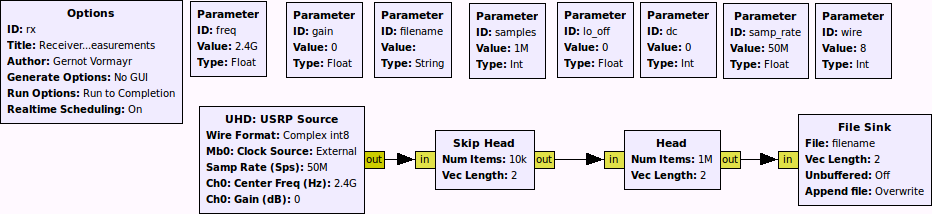
\includegraphics[width=\linewidth]{grc}
    \caption{GNU Radio companion \gls{rx} flowgraph}
    \label{fig:grc_rx}
\end{figure}
Every flowgraph has an {\ttfamily Options} block, which determines the name of the output module ({\ttfamily ID}),
which \gls{gui} to use for the application ({\ttfamily Generate Options}), and some optional runtime features.

{\ttfamily Parameter} blocks can be used for passing values from either a calling flowgraph or, as has
been used in this block, for passing values via command line arguments. {\ttfamily ID} specifies the
name of the command line argument, {\ttfamily Value} an optional default, and {\ttfamily Type} the data
type of the generated variable.

Besides parameters, signal processing blocks have input and/or output ports. Those ports
can be connected from output to input. One Output can feed several inputs. Outputs and inputs
must always be connected. There are also modules featuring optional ones.

Compiling the flowgraph in \cref{fig:grc_rx} with GNU Radio Companion, creates a python script
called {\ttfamily rx.py}, that samples packets from an \gls{usrp} source, drops the first
\num{10e3} samples ({\ttfamily Skip Head}), and writes
them into the file named {\ttfamily filename} ({\ttfamily File Sink}). Skipping samples in the
beginning is necessary, because there is no way to detect that initialization has finished
and every subsystem is in a stable state. {\ttfamily Head}
stops processing after the specified number of samples have passed through it. This python
script can be used standalone, or be adapted to requirements, that can not be met by GNU Radio
Companion (e.g. conditionally instantiating flowgraph modules).

Although most of the signal module parameters, as can be seen in \cref{fig:grc_rx}, appear to have
numerical values, they actually reference the generic parameters. GNU Radio Companion always displays the
default values of variables and parameters, if there are any.

\subsubsection{Generated Scripts}
\label{sec:radioscripts}
\begin{figure}[htbp]
    \centering
    \begin{lstlisting}[basicstyle=\tiny,caption={Generated RX flowgraph module with modifications ({\ttfamily rx\_final.py)}},label=lst:rxfinal.py]
#!/usr/bin/env python
##################################################
# Gnuradio Python Flow Graph
# Title: Receiver for Measurements
# Author: Gernot Vormayr
# Generated: Wed Dec  3 10:00:57 2014
##################################################

from gnuradio import blocks
from gnuradio import eng_notation
from gnuradio import gr
from gnuradio import uhd
from gnuradio.eng_option import eng_option
from gnuradio.filter import firdes
from optparse import OptionParser
import time

class rx(gr.top_block): (*\label{line:classdef}*)
  def __init__(self, freq=2.4e9, gain=0, filename="", samples=1000000, lo_off=0, dc=0, samp_rate=50e6, wire=8): (*\label{line:init}*)
    gr.top_block.__init__(self, "Receiver for Measurements")
    if wire == 8: (*\label{line:w81}*)
      otw_format = "sc8"
      bs = gr.sizeof_char*2
    elif wire == 16:
      otw_format = "sc16"
      bs = gr.sizeof_short*2

    ################################################## (*\label{line:blockinst}*)
    # Blocks
    ##################################################
    self.uhd_usrp_source_0 = uhd.usrp_source(
      device_addr="addr=192.168.10.2",
      stream_args=uhd.stream_args(
        cpu_format="sc16",
        otw_format=otw_format,
        channels=range(1),
      ),
    )
    self.uhd_usrp_source_0.set_clock_source("external", 0)
    self.uhd_usrp_source_0.set_samp_rate(samp_rate)
    self.uhd_usrp_source_0.set_center_freq(uhd.tune_request(freq, lo_off), 0)
    self.uhd_usrp_source_0.set_gain(gain, 0)
    if dc == 0:
      self.uhd_usrp_source_0.set_auto_dc_offset(False) (*\label{line:dcoff1}*)
      self.uhd_usrp_source_0.set_dc_offset(0)          (*\label{line:dcoff2}*)
    self.blocks_skiphead_0 = blocks.skiphead(bs, int(samp_rate))
    if wire == 8: (*\label{line:w82}*)
      self.blocks_short_to_char_0 = blocks.short_to_char(2) (*\label{line:short}*)
    self.blocks_head_0 = blocks.head(bs, samples)
    self.blocks_file_sink_0 = blocks.file_sink(bs, filename, False)
    self.blocks_file_sink_0.set_unbuffered(False)

    ################################################## (*\label{line:conninst}*)
    # Connections
    ##################################################
    if wire == 8: (*\label{line:w83}*)
      self.connect((self.uhd_usrp_source_0, 0), (self.blocks_short_to_char_0, 0))
      self.connect((self.blocks_short_to_char_0, 0), (self.blocks_skiphead_0, 0))
    elif wire == 16:
      self.connect((self.uhd_usrp_source_0, 0), (self.blocks_skiphead_0, 0))
    self.connect((self.blocks_skiphead_0, 0), (self.blocks_head_0, 0))
    self.connect((self.blocks_head_0, 0), (self.blocks_file_sink_0, 0))
(*\label{line:setters}*)
if __name__ == '__main__': (*\label{line:main}*)
  parser = OptionParser(option_class=eng_option, usage="%prog: [options]")
  parser.add_option("", "--freq", dest="freq", type="eng_float", default=eng_notation.num_to_str(2.4e9), help="Set freq [default=%default]")
  parser.add_option("", "--gain", dest="gain", type="eng_float", default=eng_notation.num_to_str(0), help="Set gain [default=%default]")
  parser.add_option("", "--filename", dest="filename", type="string", default="", help="Set filename [default=%default]")
  parser.add_option("", "--samples", dest="samples", type="intx", default=1000000, help="Set samples [default=%default]")
  parser.add_option("", "--lo-off", dest="lo_off", type="eng_float", default=eng_notation.num_to_str(0), help="Set lo_off [default=%default]")
  parser.add_option("", "--dc", dest="dc", type="intx", default=0, help="Set dc [default=%default]")
  parser.add_option("", "--samp-rate", dest="samp_rate", type="eng_float", default=eng_notation.num_to_str(50e6), help="Set samp_rate [default=%default]")
  parser.add_option("", "--wire", dest="wire", type="intx", default=8, help="Set wire [default=%default]")
  (options, args) = parser.parse_args()
  if gr.enable_realtime_scheduling() != gr.RT_OK:
    print "Error: failed to enable realtime scheduling."
  tb = rx(freq=options.freq, gain=options.gain, filename=options.filename, samples=options.samples, lo_off=options.lo_off, dc=options.dc, samp_rate=options.samp_rate, wire=options.wire)
  tb.start() (*\label{line:start}*)
  tb.wait() (*\label{line:wait}*)
    \end{lstlisting}
\end{figure}
The generated scripts follow a predefined structure. The following explains
this structure and possible entrypoints based on the script in
\cref{lst:rxfinal.py}. This script has been generated from the flowgraph
in \cref{fig:grc_rx} and modified to support additional features.

All the generated scripts contain a class (\cref{line:classdef}), which represents the flowgraph
and is named according to the {\texttt id} in the {\texttt Options} block. In the
\lstinline{__init__} function (\cref{line:init}) the whole flowgraph,
starting with the blocks (\cref{line:blockinst}) followed by the connections
(\cref{line:conninst}), is instantiated. Normally GNU Radio Companion would insert get- and set-functions for all
variables in \cref{line:setters}. Those have been removed for clarity from the
script. They are only needed if the settings need to be changed during runtime.
This can happen e.g. by changing a slider or pressing a button in the
\gls{gui}.

\Cref{line:dcoff1} and \cref{line:dcoff2} in \cref{lst:rxfinal.py} are intended to turn off \gls{dc} offset
compensation by disabling the accumulator and setting the accumulator value to zero 
(see \cref{sec:dsprx}). These two settings are not available in the GNU Radio Companion and can only
be modified from python.

Several other modifications (\Cref{line:w81,line:w82,line:w83} in \cref{lst:rxfinal.py})
make the flowgraph more dynamic, to support \SI{8}{\bit} and \SI{16}{\bit} mode with
the same python script. In \SI{8}{\bit} mode an additional block in \cref{line:short}
is added to the flowgraph, for converting the samples provided by the \gls{usrp} source
to the appropriate data type. This is necessary, because the \gls{usrp} block has a
very limited number of output data formats.

The last block in the file represents the main function (\cref{line:main}),
which is executed, when the script is called directly, instead of being
used as a module. This block parses the arguments handed over to the script,
does the necessary setup, instantiates the defined class, starts the processing
(\cref{line:start}) asynchronously, and waits for completion (\cref{line:wait}).
\lstinline{tb.stop()} could be used between those two functions to
stop processing early.

\begin{figure}[htbp]
    \centering
    \begin{lstlisting}[basicstyle=\tiny,caption={Excerpt from ({\ttfamily tx\_final.py)} demonstrating stop.},label=lst:txfinal.py]
    (*\centerline{\raisebox{-1pt}[0pt][0pt]{$\vdots$}}*)
  tb.start()
  if options.samples == 0:
    raw_input() 
    tb.stop()
  tb.wait()
  \end{lstlisting}
\end{figure}

The script {\texttt tx\_final.py} provided in \cref{sec:sources} has been
developed to send samples to the \gls{usrp}. If the number of requested
output samples is zero, samples get continously streamed. It works similar
to the script in \cref{lst:rxfinal.py} except for the startup
(see \cref{lst:txfinal.py}). After starting the flowgraph, in case of continuous
streaming mode, the script waits with \lstinline{raw_input()}
for a new line on standard input. After this happens the processing is stopped
using \lstinline{tb.stop()}. Note that \lstinline{tb.wait()} needs to be called
in this case too, because this waits for a clean shut down.

\subsection{Using the \glsentryshort{usrp} from Mathworks Matlab}
\label{sec:matlab}

Drivers that enable using the \gls{usrp} from within Matlab and Simulink are
provided by Mathworks \cite{matlab_usrp}. These drivers need Matlab's Communications
System Toolbox. The drivers only support basic functionality, like setting the center frequency
or the decimation rate. It is not possible to set the clock source of the
\gls{usrp} to external, which is needed for typical \gls{rf} measurements to
synchronize the instruments. Another problem which occured during validation of the drivers was, that Matlab
was too slow for real time data processing at a sample rate of up to
\SI{50}{\mega\samples\per\second}.

\begin{figure}[htb]
    \centering
    \begin{lstlisting}[language=matlab,basicstyle=\tiny,caption={Matlab \gls{usrp} \gls{rx} function ({\ttfamily usrp\_rx.m)}},label=lst:usrprx.m]
function [v, status] = usrp_rx(frequency, gain, samples, lo, dc, samp_rate, wire)
narginchk(3, 7); (*\label{line:argstart}*)
    if nargin < 4
        lo = 0;
    end
    if nargin < 5
        dc = 0;
    end
    if nargin < 6
        samp_rate = 50e6;
    end
    if nargin < 7
        wire = 8;
    end (*\label{line:argstop}*)
    tmp = '/run/shm/sink'; (*\label{line:tmp}*)
    cmd = sprintf('./rx_final.py --freq=%g --gain=%g --samples=%d --filename=%s --lo-off=%g --dc=%d --samp-rate=%g --wire=%d', frequency, gain, samples, tmp, lo, dc, samp_rate, wire);
    [status, result] = system(cmd);
    result = strsplit(result, '\n'); (*\label{line:check1}*)
    status = status + length(result{end}); (*\label{line:check2}*)
    v = load_data(tmp, samples, wire);
    delete(tmp);
end
    \end{lstlisting}
\end{figure}

This led to the approach of using GNU Radio for communicating with the \gls{usrp}. A
set of functions were developed, that call the scripts from \cref{sec:radioscripts}.
The \gls{rx} script, provided in \cref{lst:usrprx.m} starts with setting
default values for the arguments (\crefrange{line:argstart}{line:argstop}). To prevent
adding latencies by writing the data to disk, the sample file gets stored in
\texttt{/run/shm}, which resides in \gls{ram} (\cref{line:tmp}). This will
work under linux only. Since overruns get only reported to standard output by
GNU Radio, \cref{line:check1,line:check2} count the number of characters in
the last line of the output and add it to \texttt{status}. If \texttt{status}
is non zero, then the returned data should not be used.

\begin{figure}[htb]
    \centering
    \begin{lstlisting}[language=matlab,basicstyle=\tiny,caption={Matlab function for loading data exported by GNU Radio ({\ttfamily load\_data.m)}},label=lst:load.m]
function v = load_data(filename, count, wire)
    switch wire
        case 8
            wire = 'int8';
        case 16
            wire = 'int16';
    end
    f = fopen(filename, 'rb');
    t = fread(f, [2, count], wire);
    v = t(1,:) + t(2,:)*1i;
    [r, c] = size(v);
    v = reshape(v, c, r);
    fclose(f);
end
    \end{lstlisting}
\end{figure}

Converting the data is handled by \cref{lst:load.m}. Data from the script is
stored in binary, with I and Q samples interleaved. This function returns the
samples as a vector of complex numbers.

Functions for transmitting samples were also developed and can be found in
\cref{sec:sources}. These functions are similar to the \gls{rx} version. The
only added feature is a flag which enables asynchronously transmitting samples. This
enables doing measurements from Matlab, while transmitting.

\clearpage
%======================================================================
\section{Measurements}
\label{sec:measurements}
The \gls{usrp} needs a very high bandwidth of up to \SI{800}{\mega\bit\per\second} at \SI{50}{\mega\samples\per\second}
(without protocol overhead). To minimize packet drops on the link, every measurement setup
used a dedicated network card directly connected to the \gls{usrp}.
A list of the used instruments can be found in \cref{sec:meters}.

To automate the measurements, Matlab scripts were developed. Those scripts used the GNU Radio
flowgraphs described in \cref{sec:intgnu} using the method described in \cref{sec:matlab}. The high
data rates, caused by the high sampling rates of up to \SI{50}{\mega\samples\per\second}, would
require too much disk space for storing all the samples. Because of this samples are preprocessed
immediately after acquisition and only those preprocessed values are stored for later use.

All the measurements were taken with an uncalibrated device, to not distort the measurements
and be able to see the effects.

\subsection{RF Frequency Response}
\subsubsection{RX}
\label{sec:rfrx}
\begin{figure}[htb]
    \centering
    \begin{tikzpicture}
        \draw node[dut] (dut) {};
        \draw node[right=of dut,attenuator,label=below:\SI{6}{\deci\bel}] (att) {};
        \draw node[right=of att,generator] (src) {};
        \draw node[draw,rounded corners,below=of dut] (meas) {\begin{tabular}{l}PC \\ Matlab\end{tabular}};

        \draw[dashed] (meas) -- (dut);
        \draw (meas.north) node[anchor=south east] {\tiny eth0};
        \draw[rounded corners,dashed] (meas) -| (src);
        \draw (meas.east) node[anchor=south west] {\tiny eth1};
        \draw[open triangle 45-] (dut) -- (att);
        \draw (dut.east) node[anchor=south west] {\tiny RX};
        \draw[open triangle 45-] (att) -- (src);
    \end{tikzpicture}
    \caption{\gls{rx} \gls{rf} response measurement setup}
    \label{fig:rxrfsetup}
\end{figure}

The measurement setup can be seen in \cref{fig:rxrfsetup}. The \SI{6}{\deci\bel}
attenuator was used for protecting the \gls{usrp} and building a forced match.

As mentioned in \cref{sec:usrp} the design of the analog \gls{rx} path is missing \gls{ac}
coupling. This results in a noticeable \gls{dc} offset in the measured samples.
\gls{dc} offset compensation can completely remove this offset, but this would
also remove any \gls{if} components at \SI{0}{\hertz}. Because of this, the
\gls{rf} response was measured at an \gls{if} frequency of
\SI{1}{\mega\hertz}.

The measurements were performed with gain settings from \SI{0}{\deci\bel} to
\SI{50}{\deci\bel} in \SI{5}{\deci\bel} steps. Output power of the generator
was initially set to \SI{-14}{\deci\belm}. At each gain step the output
power was adjusted by the gain, to keep the input power to Part B in \cref{fig:usrp} constant.
For every gain setting the frequency was swept from \SI{400}{\mega\hertz} to \SI{4.4}{\giga\hertz} in
\SI{50}{\mega\hertz} steps. The line format used was \SI{8}{\bit} at
\SI{50}{\mega\samples\per\second}.

These measurements were repeated with a power meter in place of the
\gls{usrp} and the \gls{usrp} data converted as if the \SI{-14}{\deci\bel}
were present at the input. The measured data was normalized to
\SI{0}{\deci\belfs} to create the plot in \cref{fig:inputfscrf}.
This plot depicts the gain needed to reach \SI{0}{\deci\belfs} at selected center frequencies.

\begin{figure}[htb]
    \centering
\begin{tikzpicture}
    \begin{axis}[
        xlabel={gain setting},
        ylabel={input power},
        x unit={\deci\bel},
        y unit={\deci\belm},
        minor tick num = 1
        ]
        \addplot[mark = +,red] table {data/rf/rx/8/dbm_400};
        \addlegendentry{\SI{400}{MHz}}
        \addplot[mark = x,green] table {data/rf/rx/8/dbm_2400};
        \addlegendentry{\SI{2.4}{GHz}}
        \addplot[mark = asterisk,blue] table {data/rf/rx/8/dbm_4400};
        \addlegendentry{\SI{4.4}{GHz}}
    \end{axis}
\end{tikzpicture}
    \caption{Input power needed for \SI{0}{\deci\belfs} at selected center frequencies}
    \label{fig:inputfscrf}
\end{figure}

\begin{figure}[htb]
    \centering
\begin{tikzpicture}
    \begin{axis}[
        ylabel={ADC power},
        xlabel={frequency},
        y unit={\deci\belfs},
        x unit={\hertz},
        change x base,
        x SI prefix=giga,
        width=\linewidth,
        height=7cm,
        minor tick num = 1
        ]
        \addplot[black] table {data/rf/rx/8/f0_0};
    \end{axis}
\end{tikzpicture}
    \caption{\gls{adc} power over frequency at \SI{-14}{\deci\belm} input power and \SI{0}{\deci\bel} gain}
    \label{fig:gainfscrf}
\end{figure}

As can been seen in \cref{fig:inputfscrf} the gain setting of the \gls{usrp} scales nearly
linear up to \SI{30}{\deci\belm}. Higher gain values do not increase the power, because
the maximum setting is \SI{31.5}{\deci\belm}. The host driver saturates the gain setting
at the maximum setting.

According to the datasheet of the DEMOD \cite{demod} (see \cref{fig:usrp}), it
causes a part of the ripple seen in \cref{fig:gainfscrf}. The rest of the ripple is
probably caused by a mismatch of the individual consecutive components.

The power difference between \SI{400}{\mega\hertz} and \SI{4.4}{\giga\hertz}
stems in big parts from LNA1 and LNA2 \cite{rxlna}, and from the DEMOD. Other
causes can be mismatch between the components, and the filter LP1, which is only
active at lower frequencies. This results in a lower \gls{lo} power at the DEMOD.

\subsubsection{TX}
\label{sec:rftx}
\begin{figure}[htb]
    \centering
    \begin{tikzpicture}
        \draw node[dut] (dut) {};
        \draw node[right=of dut,attenuator,label=below:\SI{16}{\deci\bel}] (att) {};
        \draw node[right=of att,powermeter] (dst) {};
        \draw node[draw,rounded corners,below=of dut] (meas) {\begin{tabular}{l}PC \\ Matlab\end{tabular}};

        \draw[dashed] (meas) -- (dut);
        \draw (meas.north) node[anchor=south east] {\tiny eth0};
        \draw[rounded corners,dashed] (meas) -| (dst);
        \draw (meas.east) node[anchor=south west] {\tiny eth1};
        \draw[-open triangle 45] (dut) -- (att);
        \draw (dut.east) node[anchor=south west] {\tiny TX};
        \draw[-open triangle 45] (att) -- (dst);
    \end{tikzpicture}
    \caption{\gls{tx} \gls{rf} response measurement setup}
    \label{fig:txrfsetup}
\end{figure}

The setup to evaluate the \gls{tx} \gls{rf} response can be seen in \cref{fig:txrfsetup}.
This setup uses a \SI{16}{\deci\bel} attenuator, to limit the output signal from the \gls{usrp}
to not exceed \SI{20}{\deci\belm}. This was needed, to stay withing the acceptable range
of the used power sensor (see \cref{sec:meters}).

Measurements were taken at gain settings ranging from \SI{0}{\deci\bel} to \SI{30}{\deci\bel}
in \SI{5}{\deci\bel} steps. An additional measurement was taken at the maximal gain
setting of \SI{31.5}{\deci\bel}. \gls{rf} frequencies ranged from \SI{400}{\mega\hertz} to
\SI{4.4}{\giga\hertz} in \SI{50}{\mega\hertz} steps. The line format used was
\SI{8}{\bit} at a sampling rate of \SI{50}{\mega\samples\per\second}. In order to stay
in the linear region of \gls{dac} the generated samples had an amplitude
of $0.8 \times \text{full scale}$.

To get the results at the output port of the \gls{usrp}, the measurement data was corrected
by the insertion loss of the cable with the attenuator attached, which was measured
with a network analyzer.

\clearpage

\begin{figure}[htb]
    \centering
\begin{tikzpicture}
    \begin{axis}[
        ylabel={output power},
        xlabel={frequency},
        y unit={\deci\belm},
        x unit={\hertz},
        change x base,
        x SI prefix=giga,
        width=\linewidth,
        height=7cm,
        minor tick num = 1,
        ]
        \addplot[black] table {data/rf/tx/0.821.0/0.0};
    \end{axis}
\end{tikzpicture}
\caption{Output power over frequency, \SI{0}{\deci\belfs}, \SI{0}{\deci\bel} gain}
    \label{fig:outputrf08}
\end{figure}

Measurement results in \cref{fig:outputrf08} were normalized as if the measurement
was taken at full scale, to be able to compare this data to other measurements.
The frequency response shows a large gain droop, which, according to the datasheets
is mainly caused by AMP2\cite{amp2} and AMP3\cite{amp3} (see \cref{fig:usrp}).

\begin{figure}[htb]
    \begin{subfigure}[t]{.5\linewidth}
        \centering
\begin{tikzpicture}
    \begin{axis}[
        ylabel={output power},
        xlabel={gain setting},
        y unit={\deci\belm},
        x unit={\deci\bel},
        width=\linewidth
        ]
        \addplot[black] table {data/rf/tx/1db/1.00};
    \end{axis}
\end{tikzpicture}
    \caption{\SI{1}{\giga\hertz}}
    \label{fig:outputrf1}
    \end{subfigure}
    \begin{subfigure}[t]{.5\linewidth}
        \centering
\begin{tikzpicture}
    \begin{axis}[
        ylabel={output power},
        xlabel={gain setting},
        y unit={\deci\belm},
        x unit={\deci\bel},
        width=\linewidth
        ]
        \addplot[black] table {data/rf/tx/1db/4.00};
    \end{axis}
\end{tikzpicture}
    \caption{\SI{4}{\giga\hertz}}
    \label{fig:outputrf4}
    \end{subfigure}
    \caption{Output power over gain, \SI{0}{\deci\belfs} at two different \gls{rf} frequencies}
\end{figure}


Data shown in \cref{fig:outputrf1,fig:outputrf4} was corrected to \SI{0}{\deci\belfs}. The
two graphs visualized output power over gain. While in \cref{fig:outputrf1} compression
is noticeable, \cref{fig:outputrf4} is nearly linear. Since only ATT2 attenuation was
changed during measurements, this means the compression can only be caused by Part A
in \cref{fig:usrp}.

\subsection{IF Frequency Response}
\subsubsection{RX}
\label{sec:ifrx}
\begin{figure}[htb]
    \centering
    \begin{tikzpicture}
        \draw node[dut] (dut) {};
        \draw node[right=of dut,generator] (src) {};
        \draw node[draw,rounded corners,below=of dut] (meas) {\begin{tabular}{l}PC \\ Matlab\end{tabular}};

        \draw[dashed] (meas) -- (dut);
        \draw (meas.north) node[anchor=south east] {\tiny eth0};
        \draw[rounded corners,dashed] (meas) -| (src);
        \draw (meas.east) node[anchor=south west] {\tiny eth1};
        \draw[open triangle 45-] (dut) -- (src);
        \draw (dut.east) node[anchor=south west] {\tiny RX};
    \end{tikzpicture}
    \caption{\gls{rx} \gls{if} response measurement setup}
    \label{fig:rxifsetup}
\end{figure}

The measurement setup depicted in \cref{fig:rxifsetup} consists of a signal source, directly
connected to the \gls{usrp}. In order to ignore peaks, caused by aliasing and IQ imbalance,
the signal power of the frequencies of interest were calculated with the Matlab function
\lstinline[language=matlab]{bandpower}. This function calculates the power contained in
a signal within a specific window in the spectrum. A \SI{100}{\kilo\hertz} window was
used for this measurements.

Measurements were taken at \SI{50}{\mega\samples\per\second} and \SI{25}{\mega\samples\per\second}.
\gls{if} frequencies used for \SI{50}{\mega\samples\per\second} were \SI{-24}{\mega\hertz}
to \SI{+24}{\mega\hertz} in \SI{1}{\mega\hertz} steps, and \SI{-12}{\mega\hertz}
to \SI{+12}{\mega\hertz} in \SI{0.5}{\mega\hertz} steps for \SI{25}{\mega\samples\per\second}.
Every \gls{if} frequency response measurement was taken at center frequencies from \SI{400}{\mega\hertz}
to \SI{4.4}{\giga\hertz} in \SI{100}{\mega\hertz} steps. Those measurements were repeated
at gain settings of \SI{0}{\deci\bel}, \SI{15}{\deci\bel} and \SI{31.5}{\deci\bel}. The signal source was
initially set to \SI{-10}{\deci\belm} for the gain setting of \SI{0}{\deci\bel} and adjusted with the
gain setting for the other measurements, to keep the power constant at Part B in \cref{fig:usrp}.


\begin{figure}[htb]
    \centering
\begin{tikzpicture}
    \begin{axis}[
        ylabel={IF frequency},
        xlabel={RF frequency},
        zlabel={ADC power},
        xlabel style={sloped},
        ylabel style={sloped},
        x unit={\hertz},
        change x base,
        x SI prefix=giga,
        y unit={\hertz},
        change y base,
        y SI prefix=mega,
        z unit={\deci\belfs},
        width=\linewidth,
        height=7cm,
        minor tick num = 1,
        ]
        \addplot3[surf,mesh/cols=41] table {data/if/rx/mesh16_15.0};
    \end{axis}
\end{tikzpicture}
    \caption{\gls{adc} power, \SI{16}{\bit}, \SI{15}{\deci\bel} gain, \SI{25}{\mega\samples\per\second}}
    \label{fig:rfifrx16}
\end{figure}

For calibration, a power meter was used in place of the \gls{usrp} and the measurement
data corrected as if the chosen power setting was present at the input port.

An overview of the measurement results can be seen in \cref{fig:rfifrx16}. The slope and ripple
in the \gls{rf} frequency axis is uniformly distributed along the \gls{if} frequency axis.
These results and different gain settings, which can be found in the \cref{sec:sources},
reproduce the same result as has been observed in the \gls{rf} frequency response (see \cref{sec:rfrx}).

Since these measurements were taken without \gls{dc} offset compensation, there is a small peak at 
\SI{0}{\mega\hertz} \gls{if}, which is caused by DEMOD (see \cref{sec:dsprx}).

\begin{figure}[htb]
    \centering
\begin{tikzpicture}
    \begin{axis}[
        legend style={at={(0.5,0.03)},anchor=south},
        xlabel={IF frequency},
        ylabel={ADC power},
        x unit={\hertz},
        change x base,
        x SI prefix=mega,
        y unit={\deci\belfs},
        width=\linewidth,
        height=5cm,
        minor tick num = 1,
        xmin=-25e6,
        xmax=25e6
        ]
        \addplot[red] table {data/if/rx/16_2000_15.0};
        \addlegendentry{\SI{16}{\bit}}
        \addplot[green] table {data/if/rx/825_2000_15.0};
        \addlegendentry{\SI{8}{\bit}}
    \end{axis}
\end{tikzpicture}
    \caption{\gls{adc} power, \SI{15}{\deci\bel} gain, \gls{rf} frequency \SI{2}{\giga\hertz}, \SI{25}{\mega\samples\per\second}}
    \label{fig:ifrx25}
\end{figure}

A more detailed visualization at a single center frequency of \SI{2}{\giga\hertz}
can be seen in \cref{fig:ifrx25}. As can be seen in the graph, there are no
differences, except for the resolution, between \SI{8}{\bit} and \SI{16}{\bit}. This
is expected, since digital signal processing is the same, regardless of the bit width
(see \cref{sec:dsprx}).

The slightly sloped graph in \cref{fig:ifrx25} is probably caused by \gls{iq} imbalance,
while the cut off at the edges of the usable spectrum is caused by the alias filters.

\begin{figure}[htb]
    \centering
\begin{tikzpicture}
    \begin{axis}[
        xlabel={IF frequency},
        ylabel={ADC power},
        x unit={\hertz},
        change x base,
        x SI prefix=mega,
        y unit={\deci\belfs},
        width=\linewidth,
        height=5cm,
        minor tick num = 1,
        xmin=-25e6,
        xmax=25e6
        ]
        \addplot[red] table {data/if/rx/8_2000_15.0};
    \end{axis}
\end{tikzpicture}
    \caption{\gls{adc} power, \SI{16}{\bit}, \SI{15}{\deci\bel} gain, RF frequency \SI{2}{\giga\hertz}, \SI{50}{\mega\samples\per\second}}
    \label{fig:ifrx50}
\end{figure}

\Cref{fig:ifrx50} is a visualization of the measured data at the same center frequency
as \cref{fig:ifrx25}, but at \SI{50}{\mega\samples\per\second}. There are only
data points for \SI{8}{\bit}, because it is not possible to use \SI{16}{\bit} mode
at \SI{50}{\mega\samples\per\second} (see \cref{sec:usrp}).

In \cref{fig:ifrx50} the cut off frequency of \SI{20}{\mega\hertz}, of the LP3
filter, mentioned in \cref{sec:usrp}, is observable. The \gls{cic} roll off can also be seen, because
in \SI{50}{\mega\samples\per\second} mode only one of the half band filters is
active (see \cref{sec:dsprx}). Because of this, it can be seen that the \gls{cic} filter is not
fully compensated.

\subsubsection{TX}
\label{sec:iftx}
\begin{figure}[htb]
    \centering
    \begin{tikzpicture}
        \draw node[dut] (dut) {};
        \draw node[right=of dut,attenuator,label=below:\SI{16}{\deci\bel}] (att) {};
        \draw node[right=of att,spectrum analyzer] (dst) {};
        \draw node[draw,rounded corners,below=of dut] (meas) {\begin{tabular}{l}PC \\ Matlab\end{tabular}};

        \draw[dashed] (meas) -- (dut);
        \draw (meas.north) node[anchor=south east] {\tiny eth0};
        \draw[rounded corners,dashed] (meas) -| (dst);
        \draw (meas.east) node[anchor=south west] {\tiny eth1};
        \draw[-open triangle 45] (dut) -- (att);
        \draw (dut.east) node[anchor=south west] {\tiny TX};
        \draw[-open triangle 45] (att) -- (dst);
    \end{tikzpicture}
    \caption{\gls{tx} \gls{if} response measurement setup}
    \label{fig:txifsetup}
\end{figure}

The setup for measuring the \gls{tx} \gls{if} response can be seen in
\cref{fig:txifsetup}. For power measurements a spectrum analyzer has been used
instead of a power sensor, to measure only the targeted \gls{if} frequency. This
is needed, because significant aliasing peaks can be observed while measuring
frequencies at the edge of the usable frequency band.

\begin{figure}[htb]
    \centering
\begin{tikzpicture}
    \begin{axis}[
        ylabel={IF frequency},
        xlabel={RF frequency},
        zlabel={output power},
        xlabel style={sloped},
        ylabel style={sloped},
        x unit={\hertz},
        change x base,
        x SI prefix=giga,
        y unit={\hertz},
        change y base,
        y SI prefix=mega,
        z unit={\deci\belm},
        width=\linewidth,
        height=7cm,
        minor tick num = 1,
        restrict y to domain=-12e6:12e6,
        ]
        \addplot3[surf,mesh/cols=41] table {data/if/tx/mesh16_15.0};
    \end{axis}
\end{tikzpicture}
\caption{Output power at $0.7 \times \text{full scale}$, \SI{16}{\bit}, \SI{15}{\deci\bel} gain, \SI{25}{\mega\samples\per\second}}
    \label{fig:rfiftx16}
\end{figure}

Calibrating the spectrum analyzer was done using a power meter instead of the
spectrum analyzer and measuring a single \gls{if} frequency at
\SI{1}{\mega\hertz} for every center frequency. The samples were corrected
by the power difference between those two measurements and by the forward
transfer function of the cable, measured with a network analyzer.

The overview in \cref{fig:rfiftx16} reproduces the same slope and ripple
along the \gls{rf} frequency axis as can be seen in the \gls{rf} frequency response
(see \cref{sec:rftx}). Both are uniformly distributed along the \gls{if} frequency axis.

\begin{figure}[htb]
    \centering
\begin{tikzpicture}
    \begin{axis}[
        xlabel={IF frequency},
        ylabel={output power},
        x unit={\hertz},
        change x base,
        x SI prefix=mega,
        y unit={\deci\belm},
        width=\linewidth,
        height=5cm,
        minor tick num = 1,
        restrict x to domain=-12e6:12e6,
        xmin=-25e6,
        xmax=25e6
        ]
        \addplot[red] table {data/if/tx/16_2000_15.0};
    \end{axis}
\end{tikzpicture}
    \caption{Output power at $0.7 \times \text{full scale}$, \SI{15}{\deci\bel} gain, RF frequency \SI{2}{\giga\hertz}, \SI{25}{\mega\samples\per\second}, \SI{16}{\bit}}
    \label{fig:iftx}
\end{figure}

\Cref{fig:iftx} features only the \SI{16}{\bit} measurement, because the \SI{8}{\bit}
measurement produced the same result. Like in \cref{sec:iftx} the cut off frequency
of the aliasing filter is visible. \gls{cic} roll off is noticeable in
\SI{25}{\mega\samples\per\second}, which means, that the half band filters don't fully
compensate the \gls{cic} (see \cref{sec:dsptx}).

\begin{figure}[htb]
    \centering
\begin{tikzpicture}
    \begin{axis}[
        xlabel={IF frequency},
        ylabel={output power},
        x unit={\hertz},
        change x base,
        x SI prefix=mega,
        y unit={\deci\belm},
        width=\linewidth,
        height=5cm,
        minor tick num = 1,
        restrict x to domain=-24e6:24e6,
        xmin=-25e6,
        xmax=25e6
        ]
        \addplot[red] table {data/if/tx/8_2000_15.0};
    \end{axis}
\end{tikzpicture}
    \caption{Output power at $0.7 \times \text{full scale}$, \SI{15}{\deci\bel} gain, RF frequency \SI{2}{\giga\hertz}, \SI{50}{\mega\samples\per\second}, \SI{8}{\bit}}
    \label{fig:iftx50}
\end{figure}

Since in \SI{50}{\mega\samples\per\second} mode only one half band filter
is active (see \cref{sec:dsptx}), \gls{cic} roll of is more noticeable in
\cref{fig:iftx50} than in \cref{fig:iftx}. In \cref{fig:iftx50} the effect
of the filter LP5, which has a cut off frequency of \SI{20}{\mega\hertz}
mentioned in \cref{sec:usrp} is also observable.

\subsection{Intermodulation Properties}
\subsubsection{RX}
\label{sec:iprx}
\begin{figure}[htb]
    \centering
    \begin{tikzpicture}
        \draw node[dut] (dut) {};
        \draw node[splitter,right=of dut] (split) {};
        \draw node[attenuator,right=of split.north east,yshift=1mm,label=above:\SI{10}{\deci\bel}] (att1) {};
        \draw node[attenuator,right=of split.south east,yshift=-1mm,label=below:\SI{10}{\deci\bel}] (att2) {};
        \draw node[dc block,right=of att1] (dc1) {};
        \draw node[dc block,right=of att2] (dc2) {};
        \draw node[generator,right=of dc1] (src1) {};
        \draw node[generator,right=of dc2] (src2) {};
        \draw node[coordinate,right=of src2] (sw) {};

        \draw node[draw,rounded corners,below=of dut] (meas) {\begin{tabular}{l}PC \\ Matlab\end{tabular}};


        \draw[dashed] (meas) -- (dut);
        \draw (meas.north) node[anchor=south east] {\tiny eth0};
        \draw[rounded corners,dashed] (meas) -| (sw) -- (src2);
        \draw[rounded corners,dashed] (sw) |- (src1);
        \draw (meas.east) node[anchor=south west] {\tiny eth1};

        \draw[open triangle 45-] (dut) -- (split.A1);
        \foreach \i in {1,2}
        {
            \draw[open triangle 45-] (split.B\i) -| ($(split)!.5!(att\i)$) |- (att\i.A);
            \draw[open triangle 45-] (att\i) -- (dc\i);
            \draw[open triangle 45-] (dc\i) -- (src\i);
        }

        \draw (dut.east) node[anchor=south west] {\tiny RX};
    \end{tikzpicture}
    \caption{\gls{rx} IP3 measurement setup}
    \label{fig:rxipsetup}
\end{figure}

At first the same measurement setup as in \cref{fig:rxifsetup} was attempted,
but it was not possible to generate a signal almost free of intermodulation products with
the used vector generator (see \cref{sec:meters}) as needed for high dynamic intermodulation
measurements.

This led to the setup in \cref{fig:rxipsetup}. This setup utilized a resistive power
splitter/combiner, to combine the signals from the two generators. To prevent the signal
generators from interfering with each other, an additional \gls{dc} block and a
\SI{10}{\deci\bel} attenuator were used. Without these precautions, the generators
might detect the output of the other one and therefor lower the output power, because
of internal power leveling. This is the case, because resistive power splitters
have very poor isolation of around \SI{6}{\deci\bel}.

The \gls{usrp} was set to a center frequency of \SI{1}{\giga\hertz}, one generator
to $\SI{1}{\giga\hertz} + \SI{0.5}{\mega\hertz}$ and the other one to $\SI{1}{\giga\hertz}
- \SI{0.5}{\mega\hertz}$. In order to keep the intermodulation products independent of the
phase, the generators were not synchronized. These frequency settings result in third order
intermodulation products at $\SI{1}{\giga\hertz} + \SI{1.5}{\mega\hertz}$ and
$\SI{1}{\giga\hertz} - \SI{1.5}{\mega\hertz}$. The power of the spectral components was
measured with the Matlab function \lstinline[language=matlab]{bandpower} with a window
size of \SI{100}{\kilo\hertz}. All the measurements were taken with a sample rate of \SI{25}{\mega\samples\per\second}
and \SI{16}{\bit} per sample. Measured samples were corrected by a second measurement with a power meter in place of the
\gls{usrp}, to get the power levels as if they were directly applied to the input port.

\begin{figure}[htb]
    \centering
\begin{tikzpicture}
    \begin{axis}[
        legend pos = south east,
        ylabel={adc power},
        xlabel={input power},
        y unit={\deci\belfs},
        x unit={\deci\belm},
        width=\linewidth,
        height=6cm,
        minor tick num = 1,
        ]
        \addplot[only marks, mark = +] table {data/ip3/rx/la};
        \addplot[only marks, mark = x] table {data/ip3/rx/im3};
        \addplot[only marks, mark = asterisk] table {data/ip3/rx/pim3};
        \addplot[domain = -63:-5, samples = 201,green] {1*x+33.0765};
        \addplot[domain = -63:-5, samples = 201,red] {3*x+48.2541};
        \legend{$out$,$IM_3$,$IP_3$}
    \end{axis}
\end{tikzpicture}
    \caption{\gls{rx} IP3}
    \label{fig:rxip3}
\end{figure}

Stepping the attenuation of ATT1 (see \cref{fig:usrp}) did not result in noticeable
third order intermodulation products. Decreasing the attenuation by \SI{1}{\deci\bel} increased
these products by \SI{1}{\deci\bel}. This means, that the intermodulation products shown
in \cref{fig:rxip3} are caused by Part B in \cref{fig:usrp}. Because of this, the
measurement was taken at a fixed gain setting of \SI{31.5}{\deci\bel} (ATT1 attenuation
setting of \SI{0}{\deci\bel}), while stepping the signal power.

The points in \cref{fig:rxip3} show the measured samples. $IM_3$-samples
below the input power of \SI{-43}{\deci\belm} were not increasing with the input
power, because they were below the quantization noise of the \gls{adc}. These points
could be measured by averaging over longer sample periods. The last $IM_3$ sample
with a significant higher value then the others, was taken at a higher level, then
the \gls{adc} can measure. This causes severe distortion and this value had to be
discarded.

To calculate the third order intercept point, the $out$ samples were fitted with Matlab's
Curve Fitting Toolbox to a line with a slope of one. The $IM_3$ samples were fitted to
a line with a slope of three. The point were both curves intersect is called the third order intercept point.
The calculated value for the third order input intercept point is $IIP_3 = \SI{-7.6}{\deci\belm}$
($OIP_3 = \SI{25.5}{\deci\belfs}$).

\subsubsection{TX}
\label{sec:iptx}
\begin{figure}[htb]
    \centering
    \begin{tikzpicture}
        \draw node[dut] (dut) {};
        \draw node[right=of dut,attenuator,label=below:\SI{16}{\deci\bel}] (att) {};
        \draw node[right=of att,spectrum analyzer] (dst) {};
        \draw node[draw,rounded corners,below=of dut] (meas) {\begin{tabular}{l}PC \\ Matlab\end{tabular}};

        \draw[dashed] (meas) -- (dut);
        \draw (meas.north) node[anchor=south east] {\tiny eth0};
        \draw[rounded corners,dashed] (meas) -| (dst);
        \draw (meas.east) node[anchor=south west] {\tiny eth1};
        \draw[-open triangle 45] (dut) -- (att);
        \draw (dut.east) node[anchor=south west] {\tiny TX};
        \draw[-open triangle 45] (att) -- (dst);
    \end{tikzpicture}
    \caption{\gls{tx} IP3 measurement setup}
    \label{fig:txipsetup}
\end{figure}

Measurements were taken with the setup in \cref{fig:txipsetup}. To limit the maximum output
power of the \gls{usrp}, a \SI{16}{\deci\bel} attenuator was used. This was needed to be
able to use the power sensor mentioned in \cref{sec:meters}. The power meter was used in
place of the spectrum analyzer for calibration measurements.

The \gls{usrp} was set exemplary to a center frequency of \SI{2}{\giga\hertz}. Samples for a dual
tone signal with \gls{if} frequencies of \SI{+0.5}{\mega\hertz} and \SI{-0.5}{\mega\hertz}
were sent to the \gls{usrp}. This resulted in third order intermodulation products at
\SI{+1.5}{\mega\hertz} and \SI{-1.5}{\mega\hertz} offset to the center frequency, which
were measured using a spectrum analyzer.

Since it is not possible to use two generators without modifying the \gls{usrp}, multiple
measurements with random phases were taken. Those measurements were averaged, to get results,
that are independent of the phase. All the measurements were taken with a sample rate of \SI{25}{\mega\samples\per\second}
and with \SI{16}{\bit} per sample. Measured samples were corrected by the insertion loss of the cable with the
attenuator attached, which was measured with a network analyzer.

Since changing the attenuation setting of ATT2 (see \cref{fig:usrp}) did not result in
measurable intermodulation products, the \gls{usrp} was set to a fixed gain setting of
\SI{20}{\deci\bel}. Like in \cref{sec:iprx}, decreasing the attenuation by 
\SI{1}{\deci\bel} increased the third order intermodulation products by
\SI{1}{\deci\bel}. This also means, that the intermodulation products
shown in \cref{fig:txip3} are caused by Part B in \cref{fig:usrp}.

\begin{figure}[htb]
    \centering
\begin{tikzpicture}
    \begin{axis}[
        legend pos = south east,
        ylabel={output power},
        xlabel={adc power},
        x unit={\deci\belfs},
        y unit={\deci\belm},
        width=\linewidth,
        height=6cm,
        minor tick num = 1,
        ]
        \addplot[only marks, mark = +] table {data/ip3/tx/la};
        \addplot[only marks, mark = x] table {data/ip3/tx/im3};
        \addplot[only marks, mark = asterisk] table {data/ip3/tx/pim3};
        \addplot[domain = -27:17, samples = 201,green] {1*x+25.767};
        \addplot[domain = -27:17, samples = 201,red] {3*x-3.6197};
        \legend{$out$,$IM_3$,$IP_3$}
    \end{axis}
\end{tikzpicture}
    \caption{\gls{tx} IP3}
    \label{fig:txip3}
\end{figure}

The results in \cref{fig:txip3} show the measured samples of the third order
intermodulation products ($IM_3$) and the output power ($out$). $IM_3$ samples
below \SI{-49}{\deci\belm} output power were discarded, because they were
below the noise floor.

The third order intercept point was calculated in the same way as in \cref{sec:iprx}
described. The resulting third order output intercept point is $OIP_3 = \SI{40.5}{\deci\belm}$
($IIP_3 = \SI{14.7}{\deci\belfs}$).

%======================================================================
\clearpage
\section{Conclusions}

Putting the \gls{usrp} device and GNU Radio into operation required no configuration.
This is because of the open design, which means, that every schematic and the source code is online
available. This leads to a higher number of contributors, fixing bugs
and improving the design, which wouldn't be possible that easy for a closed design. Another
reason is that the device was specifically designed for GNU Radio. One down side
of this is, that the whole platform is not a still standing target, which can cause
the drivers and the hardware to mismatch easily. Because of this always the latest
driver and hardware firmware should be used (see \cref{sec:usrp}).

Via interchangeable daughter boards, a very wide frequency range is supported by
the \gls{usrp}. In combination with up to \SI{16}{\bit} sample resolution and the
sample rate of up to \SI{50}{\mega\samples\per\second} a wide range of applications
is possible. These high sample rates imply a significant strain on the network
and computer hardware used. To achieve the best performance a dedicated network
card with a direct link should be used to connect the \gls{usrp} with the computer.
It is also advisable to shut down every unneeded software. Profiling \gls{volk},
as mentioned in \cref{sec:intgnu} is absolutely necessary.

It is also important to be aware of the difference between the Ettus Research
\gls{usrp} and the \gls{ni} version. While the Ettus Research version uses
\SI{40}{\mega\hertz} filters for LP2 and LP5 in \cref{fig:usrp}, the \gls{ni}
version uses \SI{20}{\mega\hertz} instead. This was verified in
\cref{sec:ifrx,sec:iftx} and is mentioned in a figure in \cite{ni_29xx} only.

As can be seen in \cref{sec:rfrx,sec:rftx,sec:ifrx,sec:iftx}, without calibration
there is a noticeable \gls{iq} imbalance and \gls{dc} offset. The \gls{iq} imbalance
is caused by the DEMOD for \gls{rx}, the MOD for \gls{tx}, and the tolerances
in the I and Q paths in \cref{fig:usrp}. DEMOD and MOD also cause the \gls{dc} offset,
which is not compensated in the analog hardware. Demanding radio applications
won't work with an uncalibrated device.

In the \Gls{tx} path, there is a compression at low center frequencies with high
gain settings (see \cref{fig:outputrf1}). This limits the possible output power and
linear operation dynamic range. An additional amplifier would be needed for high
power applications.

Because of the design of the \gls{ddc} and \gls{duc} chain (see
\cref{sec:dsprx,sec:dsptx}), there is noticeable \gls{cic} rolloff if only one
half band filter is active. With odd decimation rates no half band filter is
active at all and the \gls{cic} is not compensated. The driver puts out a warning
message, if this is the case. Because of this only decimation/interpolation rates
divisible by four, or an additional compensating filter should be used. The \gls{tx} shows
a slight \gls{cic} rolloff despite both half band filters being active (see
\cref{fig:iftx}). This should be verified in a future work and the filter
coefficients of the half band filters should be validated or revised.

%======================================================================
\clearpage
\begin{appendix}
\section{Measurement data and source code}
\label{sec:sources}
All the raw data, processed results and sources can be found at
\url{https://github.com/notti/usrp_measurements}.
\section{Used Instruments}
\label{sec:meters}
A Rhode \& Schwarz SMBV 100A, and a Rhode \& Schwarz SMIQ06B were used to generate
signals for RX measurements and as clock reference. Since the SMIQ06B possesses no
Ethernet connectivity, an Agilent E85810 GPIB Etheret bridge provided the necessary
conversion. Power measurements have been carried out with an Agilent N1914A Power Meter and an
Agilent E9301A averaging Power Sensor. A Rhode \& Schwarz ZVL was used to carry out
spectrum measurements and measure cable losses. \Cref{tab:meters} lists which instrument
was used for which measurement.

\begin{table}[h!]
    \centering
    \begin{tabular}{lcccccc}
        & \rot{\gls{rf} \gls{rx}} & \rot{\gls{rf} \gls{tx}} & \rot{\gls{if} \gls{rx}} & \rot{\gls{if} \gls{tx}} & \rot{IM \gls{rx}} & \rot{IM \gls{tx}} \\
        \midrule
        SMBV & \X &   &   &   & \X &   \\
        SMIQ &    &   & \X &   & \X &   \\
        Power Meter & \X & \X & \X & \X & \X & \X \\
        ZVL &    & \X &   & \X & \X & \X \\
        \bottomrule
    \end{tabular}
    \caption{Used Instruments}
    \label{tab:meters}
\end{table}

\printglossary[type=\acronymtype]

\listoffigures

\bibliographystyle{IEEEtran}
\bibliography{IEEEabrv,literature}

\section*{Copyright}
This work is licensed under the Creative Commons Attribution 4.0 International
License. To view a copy of this license, visit
\url{http://creativecommons.org/licenses/by/4.0/} or send a letter to Creative
Commons, 444 Castro Street, Suite 900, Mountain View, California, 94041, USA.

\clearpage
\section*{Code of Conduct}
Hiermit erkl\"are ich, dass die vorliegende Arbeit ohne unzul\"assige Hilfe Dritter und ohne Benutzung
anderer als der angegebenen Hilfsmittel angefertigt wurde. Die aus anderen Quellen oder indirekt
\"ubernommenen Daten und Konzepte sind unter Angabe der Quelle gekennzeichnet.
Die Arbeit wurde bisher weder im In- noch im Ausland in gleicher oder in \"ahnlicher Form in anderen
Pr\"ufungsverfahren vorgelegt.

\par\noindent\makebox[7cm]{\hrulefill}      \hfill\makebox[5cm]{\hrulefill}%
\par\noindent\makebox[7cm][l]{Unterschrift} \hfill\makebox[5cm][l]{Datum}%

\end{appendix}
\end{document}
